% This is samplepaper.tex, a sample chapter demonstrating the
% LLNCS macro package for Springer Computer Science proceedings;
% Version 2.20 of 2017/10/04
%
\documentclass[runningheads]{llncs}
%
\usepackage{graphicx,hyperref}
% Used for displaying a sample figure. If possible, figure files should
% be included in EPS format.
%
% If you use the hyperref package, please uncomment the following line
% to display URLs in blue roman font according to Springer's eBook style:
% \renewcommand\UrlFont{\color{blue}\rmfamily}
\usepackage{xcolor,xspace,amsmath,amsfonts,stmaryrd,amssymb,enumerate}
\usepackage{mathpartir}

\newcommand{\todo}[1]{\textcolor{red}{TO DO:#1}}
\newcommand{\erase}[1]{\textcolor{orange}{#1}}


%%%%%%%%%%%%%%%%%%%%%%%%%%%%%%%%%%%%%%%%%%%%%%%%%%%%%%%%%%%%%%%%%%%%%%%%%%%%%%%%%%%%%%%%%%%%%%%%%%%%
% Contents
% --------

% 1.  Formating
% 2.  Maths - Theorems
% 3.  The pi Calculus
% 4.  Session Syntax
% 5.  Subject Reduction
% 6.  Global Session Types
% 7.  Global Session Types Equivalence
% 8.  Projection
% 9.  Local Session Types
% 10. Behavioural Theory
% 11. Typed Transitions - Reductions
% 12. Typed Relations
% 13. Confluence Determinacy
% 14. Mapping
% 15. pi Constructs
% 16. LN Transform
% 17. General Types Processes Names Sessions ETC
% 18. newtheorem - newenvironment
% 19. Misc
%%%%%%%%%%%%%%%%%%%%%%%%%%%%%%%%%%%%%%%%%%%%%%%%%%%%%%%%%%%%%%%%%%%%%%%%%%%%%%%%%%%%%%%%%%%%%%%%%%%%


%%%%%%%%%%%%%%%%%%%%%%%%%%%%%%%%%%%%%%%%%%%%%%%%%%%%%%%%%%%%%%%%%%%%%%%%%%%%%%%%%%%%%%%%%%%%%%%%%%%%
%                                       FORMATING
%%%%%%%%%%%%%%%%%%%%%%%%%%%%%%%%%%%%%%%%%%%%%%%%%%%%%%%%%%%%%%%%%%%%%%%%%%%%%%%%%%%%%%%%%%%%%%%%%%%%

% Symbols
\newcommand{\semicolon}{:}
%\newcommand{\colon}{;}
\newcommand{\lrangle}[1]{\langle #1 \rangle}
\newcommand{\blrangle}[1]{\big\langle #1 \big\rangle}

%Tags
\newcommand{\parenthtext}[1]{(\textrm{\small #1})}
\newcommand{\brtext}[1]{[\textrm{\small #1}]}
\newcommand{\textinmath}[1]{\textrm{#1}}
\newcommand{\srule}[1]{\parenthtext{#1}}
\newcommand{\strule}[1]{\textrm{#1}}
\newcommand{\stypes}[1]{{\footnotesize \parenthtext{#1}}}
\newcommand{\ltsrule}[1]{{\footnotesize \lrangle{\textrm{#1}}}}
\newcommand{\eltsrule}[1]{{\footnotesize [\textrm{#1}]}}
\newcommand{\trule}[1]{{\footnotesize\brtext{#1}}}
\newcommand{\orule}[1]{{\scriptsize{\brtext{#1}}}}
\newcommand{\mrule}[1]{{\footnotesize{\parenthtext{#1}}}}

\newcommand{\iftag}{{\textrm{if }}}

% General
\newcommand{\noi}{\noindent}
\newcommand{\Hline}{\rule{\linewidth}{.5pt}}
\newcommand{\Hlinefig}{\rule{\linewidth}{.5pt}\vspace{-4mm}}
\newcommand{\myparagraph}[1]{\noindent{\textbf{#1}\ }}
\newcommand{\jparagraph}[1]{\paragraph{\textbf{#1}}}

%%%%%%%%%%%%%%%%%%%%%%%%%%%%%%%%%%%%%%%%%%%%%%%%%%%%%%%%%%%%%%%%%%%%%%%%%%%%%%%%%%%%%%%%%%%%%%%%%%%%
%                                       MATHS - THEOREMS
%%%%%%%%%%%%%%%%%%%%%%%%%%%%%%%%%%%%%%%%%%%%%%%%%%%%%%%%%%%%%%%%%%%%%%%%%%%%%%%%%%%%%%%%%%%%%%%%%%%%

%\newtheorem{notation}[definition]{Notation}

% BNF form
\newcommand{\bnfis}{\;\;::=\;\;}
%\newcommand{\bnfbar}{\;\;\;{\large |}\;\;\;}
%\newcommand{\sbnfbar}{\;|\;}
\def\bnfbar{\; \mbox{\large{$\parallel$}}\;}
\def\sbnfbar{\;\mbox{\large{$\mid$}}\;}


% Proof
\newcommand{\Case}[1]{\noi {\bf Case: }#1\\}
\newcommand{\proofend}{\qed}
%\newcommand{\proofend}{}
\newcommand{\Proof}{\noi {\bf Proof: }}

% Logic
\newcommand{\LogAnd}{\texttt{ and }}
\newcommand{\LogOr}{\texttt{ or }}

% Induction

\newcommand{\basic}{\noi {\bf Basic Step:}\\}
\newcommand{\inductive}{\noi {\bf Inductive Hypothesis:}\\}
\newcommand{\induction}{\noi {\bf Induction Step:}\\}

% Tree

\newcommand{\tree}[2]{
\ensuremath{\displaystyle
		\frac
		{
			%%\raisebox{0.0mm}{$\displaystyle{#1}$}
			#1
			%\vspace{0mm}
		}{
			%\vspace{2mm}
			#2
			%\raisebox{-0.4mm}{$\displaystyle{#2}$}
		}
	}
}


%\newcommand{\tree}[2]{
%\begin{prooftree}
%	#1
%	\justifies
%	#2
%\end{prooftree}
%}

\newcommand{\treeusing}[3]{
\begin{prooftree}
	#1
	\justifies
	#2
	\using
	#3
\end{prooftree}}

% Vectors
\newcommand{\vect}[1]{\tilde{#1}}
\newcommand{\mytilde}[1]{\widetilde{#1}}

% Functions - Set theory
\newcommand{\set}[1]{\{#1\}}
\newcommand{\es}{\emptyset}
\newcommand{\maxset}[1]{\max(#1)}
\newcommand{\setbar}{\ \ |\ \ }
\newcommand{\tuple}[2]{(#1, #2)}
\newcommand{\suchthat}{\cdot}
\newcommand{\powerset}[1]{\mathcal{P}(#1)}
\newcommand{\product}{\times}

\newcommand{\eval}{\downarrow}

\newcommand{\setsubtr}[2]{#1 \backslash #2}

\newcommand{\func}[2]{#1(#2)}
\newcommand{\dom}[1]{\mathtt{dom}(#1)}
\newcommand{\codom}[1]{\mathtt{codom}(#1)}

\newcommand{\funcbr}[2]{#1\lrangle{#2}}

\newcommand{\entails}{\text{implies}}


%%%%%%%%%%%%%%%%%%%%%%%%%%%%%%%%%%%%%%%%%%%%%%%%%%%%%%%%%%%%%%%%%%%%%%%%%%%%%%%%%%%%%%%%%%%%%%%%%%%%
%                                        pi - CALCULUS
%%%%%%%%%%%%%%%%%%%%%%%%%%%%%%%%%%%%%%%%%%%%%%%%%%%%%%%%%%%%%%%%%%%%%%%%%%%%%%%%%%%%%%%%%%%%%%%%%%%%

% Free-Bound notation
\newcommand{\freev}[1]{\lrangle{#1}}
\newcommand{\boundv}[1]{(#1)}

% General pi calculus Syntax
\newcommand{\send}[1]{\overline{#1}}
\newcommand{\ol}[1]{\overline{#1}}
\newcommand{\receive}[1]{#1.}
\newcommand{\inact}{\mathbf{0}}
\newcommand{\If}{\sessionfont{if}\ }
\newcommand{\Then}{\sessionfont{then}\ }
\newcommand{\Else}{\sessionfont{else}\ }
\newcommand{\ifthen}[2]{\If #1\ \Then #2\ }
\newcommand{\ifthenelse}[3]{\ifthen{#1}{#2} \Else #3}
\newcommand{\Par}{\;|\;}
\newcommand{\news}[1]{(\nu\, #1)}
\newcommand{\newsp}[2]{(\nu\, #1)(#2)}
\newcommand{\varp}[1]{#1}
%\newcommand{\rvar}[1]{\mathcal{#1}}
\newcommand{\rvar}[1]{#1}
%\newcommand{\rec}[2]{\mu #1. #2}
\newcommand{\recp}[2]{\mu \rvar{#1}. #2}

\newcommand{\Def}{\sessionfont{def}\ }

\newcommand{\defeq}{\stackrel{\Def}{=}}

\newcommand{\repl}{\ast\,}
\newcommand{\parcomp}[2]{\prod_{#1}{#2}}

% Free-Bound-Names sets
\newcommand{\bn}[1]{\mathtt{bn}(#1)}
\newcommand{\fn}[1]{\mathtt{fn}(#1)}
\newcommand{\sn}[1]{\mathtt{sn}(#1)}
\newcommand{\ofn}[1]{\mathsf{ofn}(#1)}
\newcommand{\fv}[1]{\mathtt{fv}(#1)}
\newcommand{\bv}[1]{\mathtt{bv}(#1)}
\newcommand{\fs}[1]{\mathtt{fs}(#1)}
\newcommand{\fpv}[1]{\mathtt{fpv}(#1)}
\newcommand{\nam}[1]{\mathtt{n}(#1)}

%Subject - Object
\newcommand{\subj}[1]{\mathtt{subj}(#1)}
\newcommand{\obj}[1]{\mathtt{obj}(#1)}

% Relations
\newcommand{\relfont}[1]{\mathcal{#1}}
\newcommand{\rel}[3]{#1\ \relfont{#2}\ #3}

\newcommand{\scong}{\equiv}
\newcommand{\acong}{\scong_{\alpha}}
\newcommand{\wb}{\approx}
\newcommand{\fwb}{\approx^\mathtt{C}}
\newcommand{\hwb}{\approx^\mathtt{H}}
\newcommand{\swb}{\approx^{s}}
\newcommand{\wbc}{\approx}
\newcommand{\WB}{\approx}

\newcommand{\red}{\longrightarrow}
\newcommand{\Red}{\rightarrow\!\!\!\!\!\rightarrow}
\newcommand{\Redleft}{\leftarrow\!\!\!\!\!\leftarrow}

%\newcommand{\subst}[2]{\set{#1/#2 }}
\def\subst#1#2{\{\raisebox{.5ex}{\small$#1$}\! / \mbox{\small$#2$}\}}

% Context
\newcommand{\hole}{-}
\newcommand{\context}[2]{#1[#2]}
\newcommand{\Ccontext}[1]{\C[#1]}

% Expression Context
\newcommand{\Econtext}[1]{\E[#1]}

% Barbs
\newcommand{\barb}[1]{\downharpoonright_{#1}}
\newcommand{\Barb}[1]{\Downarrow_{#1}}
\newcommand{\nbarb}[1]{\not\downarrow_{#1}}
\newcommand{\nBarb}[1]{\not\Downarrow_{#1}}

% General
%\newcommand{\ESP}{\ensuremath{\mathbf{ESP}}}
\newcommand{\ESP}{\text{ESP}}
\newcommand{\ESPsel}{\ESP^+}

%%%%%%%%%%%%%%%%%%%%%%%%%%%%%%%%%%%%%%%%%%%%%%%%%%%%%%%%%%%%%%%%%%%%%%%%%%%%%%%%%%%%%%%%%%%%%%%%%%%%
%                                        SESSION SYNTAX
%%%%%%%%%%%%%%%%%%%%%%%%%%%%%%%%%%%%%%%%%%%%%%%%%%%%%%%%%%%%%%%%%%%%%%%%%%%%%%%%%%%%%%%%%%%%%%%%%%%%

% Session font
\newcommand{\sessionfont}[1]{\mathtt{#1}}
\newcommand{\vart}[1]{\mathsf{#1}}

% General Session symbols
\newcommand{\ssep}{;}
\newcommand{\shsep}{.}
\newcommand{\outses}{!}
\newcommand{\inpses}{?}
\newcommand{\selses}{\triangleleft}
\newcommand{\brases}{\triangleright}
\newcommand{\dual}[1]{\overline{#1}}
\newcommand{\cat}{\cdot}

\newcommand{\allstypes}{\mathcal{S}}

% Binary Session Syntax


\newcommand{\bacc}[2]{#1 \boundv{#2} \shsep}
\newcommand{\breq}[2]{\send{#1} \freev{#2} \shsep}
\newcommand{\bareq}[2]{\send{#1} \freev{#2}}

\newcommand{\breqt}[3]{\send{#1} \boundv{#2:#3} \shsep}
\newcommand{\bacct}[3]{#1 \boundv{#2:#3} \shsep}

\newcommand{\bout}[2]{#1 \outses \freev{#2} \shsep}
\newcommand{\bbout}[2]{#1 \outses \blrangle{#2} \shsep}
\newcommand{\binp}[2]{#1 \inpses \boundv{#2} \shsep}
\newcommand{\bselold}[2]{#1 \selses #2 \shsep}
\newcommand{\bsel}[2]{#1 \selses \set{#2}}

%\newcommand{\bout}[2]{#1 \outses \freev{#2} \ssep}
%\newcommand{\bbout}[2]{#1 \outses \blrangle{#2} \ssep}
%\newcommand{\binp}[2]{#1 \inpses \boundv{#2} \ssep}
%\newcommand{\bsel}[2]{#1 \selses #2 \ssep}
\newcommand{\bbra}[2]{#1 \brases \set{#2}}
\newcommand{\bbras}[2]{#1 \brases #2}
\newcommand{\bbraP}[1]{#1 \brases \lPi}

% Multiparty Session syntax

\newcommand{\role}[1]{[#1]}

\newcommand{\srole}[2]{#1\role{#2}}
\newcommand{\sqrole}[2]{#1^{[]}\role{#2}}

\newcommand{\fromto}[2]{\role{#1} \role{#2}}
\newcommand{\sfromto}[3]{#1\fromto{#2}{#3}}

\newcommand{\sout}[3]{\srole{#1}{#2} \outses \freev{#3} \ssep}
\newcommand{\sinp}[3]{\srole{#1}{#2} \inpses \boundv{#3} \ssep}
\newcommand{\sdel}[4]{\srole{#1}{#2} \outses \freev{\srole{#3}{#4}} \ssep}
\newcommand{\ssel}[3]{\srole{#1}{#2} \selses #3 \ssep}
\newcommand{\sbra}[3]{\srole{#1}{#2} \brases \set{#3}}
\newcommand{\sbras}[3]{\srole{#1}{#2} \brases #3}
\newcommand{\sbraP}[2]{\srole{#1}{#2} \brases \lPi}

\newcommand{\acc}[3]{#1 \role{#2} \boundv{#3} \shsep}
\newcommand{\req}[3]{\send{#1} \role{#2} \boundv{#3} \shsep}
\newcommand{\areq}[3]{\send{#1} \role{#2} \freev{#3}}

\newcommand{\out}[4]{\sfromto{#1}{#2}{#3} \outses \freev{#4} \ssep}
\newcommand{\inp}[4]{\sfromto{#1}{#2}{#3} \inpses \boundv{#4} \ssep}
\newcommand{\del}[5]{\sfromto{#1}{#2}{#3} \outses \freev{\srole{#4}{#5}} \ssep}
\newcommand{\sel}[4]{\sfromto{#1}{#2}{#3} \selses #4 \ssep}
\newcommand{\bra}[4]{\sfromto{#1}{#2}{#3} \brases \set{#4}}
\newcommand{\bras}[4]{\sfromto{#1}{#2}{#3} \brases #4}
\newcommand{\braP}[3]{\sfromto{#1}{#2}{#3} \brases \lPi}

% Arrive construct
\newcommand{\arrivetext}{\mathtt{arrive}}
\newcommand{\arrive}[1]{\arrivetext\ #1}
\newcommand{\arrivem}[2]{\arrivetext\ #1\ #2}

% Typecase construct
\newcommand{\typecasetext}{\mathtt{typecase}}
\newcommand{\oftext}{\mathtt{of}}
\newcommand{\typecase}[2]{\typecasetext\ #1\ \oftext\ \set{#2}}

% IO symbols
\newcommand{\inputsym}{\mathtt{i}}
\newcommand{\outputsym}{\mathtt{o}}

%%%%%%%%%%%%%%%%%%%%%%%%%%%%%%%%%%%%%%%%%%%%%%%%%%%%%%%%%%%%%%%%%%%%%%%%%%%%%%%%%%%%%%%%%%%%%%%%%%%%
%                                      SUBJECT REDUCTION
%%%%%%%%%%%%%%%%%%%%%%%%%%%%%%%%%%%%%%%%%%%%%%%%%%%%%%%%%%%%%%%%%%%%%%%%%%%%%%%%%%%%%%%%%%%%%%%%%%%%

% typing reduction
\newcommand{\typingred}{\red}
\newcommand{\typingRed}{\Red}

\newcommand{\wellconf}[1]{\mathtt{wc}(#1)}
\newcommand{\cohses}[2]{\mathtt{co}(#1(#2))}
\newcommand{\coherent}[1]{\mathtt{co}(#1)}
\newcommand{\fcoherent}[1]{\mathtt{fco}(#1)}

%%%%%%%%%%%%%%%%%%%%%%%%%%%%%%%%%%%%%%%%%%%%%%%%%%%%%%%%%%%%%%%%%%%%%%%%%%%%%%%%%%%%%%%%%%%%%%%%%%%%
%                                      SESSION ENDPOINTS
%%%%%%%%%%%%%%%%%%%%%%%%%%%%%%%%%%%%%%%%%%%%%%%%%%%%%%%%%%%%%%%%%%%%%%%%%%%%%%%%%%%%%%%%%%%%%%%%%%%%

% Asynchronous syntax
%\newcommand{\mareq}[4]{\newsp{\srole{#2}{#3}, \dots, \srole{#2}{#4}}{\send{#1}[#3] \freev{#2} \Par \dots \Par \send{#1}[#4]\freev{#2}}}

%\newcommand{\areqs}[3]{\send{#1}[\set{#2}] \freev{#3}}

% Queues
\newcommand{\emp}{\epsilon}
\newcommand{\squeue}[3]{\srole{#1}{#2}:#3}
\newcommand{\srqueue}[4]{\srole{#1}{#2}[\inputsym: #3, \outputsym: #4]}
\newcommand{\srqueuei}[3]{\srole{#1}{#2}[\inputsym: #3]}
\newcommand{\srqueueo}[3]{\srole{#1}{#2}[\outputsym: #3]}
\newcommand{\srqueueio}[4]{\srole{#1}{#2}[\inputsym: #3, \outputsym: #4]}
\newcommand{\sgqueue}[2]{\srole{#1}:#2}

% Shared Names Queues
\newcommand{\shqueue}[2]{#1[#2]}
%\newcommand{\shqueuet}[3]{#1[#2, #3]}

% IO Queues
\newcommand{\squeueio}[3]{#1[\inputsym: #2, \outputsym: #3]}
\newcommand{\squeuei}[2]{#1[\inputsym: #2]}
\newcommand{\squeueo}[2]{#1[\outputsym: #2]}

\newcommand{\squeuetio}[4]{#1[#2, \inputsym: #3, \outputsym: #4]}
\newcommand{\squeueto}[3]{#1[#2, \outputsym: #3]}
\newcommand{\squeueti}[3]{#1[#2, \inputsym: #3]}
\newcommand{\squeuet}[2]{#1[#2]}

% Queue Values

\newcommand{\queuev}[2]{\role{#1}(#2)}
\newcommand{\queuel}[2]{\role{#1} #2}
\newcommand{\queues}[3]{\role{#1}(\srole{#2}{#3})}

%%%%%%%%%%%%%%%%%%%%%%%%%%%%%%%%%%%%%%%%%%%%%%%%%%%%%%%%%%%%%%%%%%%%%%%%%%%%%%%%%%%%%%%%%%%%%%%%%%%%
%                                        GLOBAL SESSION TYPES
%%%%%%%%%%%%%%%%%%%%%%%%%%%%%%%%%%%%%%%%%%%%%%%%%%%%%%%%%%%%%%%%%%%%%%%%%%%%%%%%%%%%%%%%%%%%%%%%%%%%

\newcommand{\impl}[2]{\{\!\{#1\}\!\}_{\mathcal{#2}}}
\newcommand{\impll}[2]{\{\!\{#1\}\!\}_{\mathcal{#2}}^\fw}

\newcommand{\gtfont}[1]{\mathtt{#1}}
\newcommand{\gsep}{.}

\newcommand{\globaltype}[1]{\lrangle{#1}}
\newcommand{\parties}[1]{\mathtt{\pa}(#1)}
\newcommand{\roles}[1]{\mathtt{roles}(#1)}

\newcommand{\fromtogt}[2]{#1 \rightarrow #2 \semicolon}

\newcommand{\valuegt}[3]{\fromtogt{#1}{#2} \lrangle{#3} \gsep}
\newcommand{\selgt}[3]{\fromtogt{#1}{#2} \set{#3}}
\newcommand{\selgtG}[2]{\fromtogt{#1}{#2} \lGi}
\newcommand{\recgt}[2]{\mu \vart{#1}. #2}
\newcommand{\vargt}[1]{\vart{#1}}
\newcommand{\inactgt}{\gtfont{end}}

\newcommand{\swap}{\ensuremath{\approx_{\mathtt{sw}}}\xspace}

%%%%%%%%%%%%%%%%%%%%%%%%%%%%%%%%%%%%%%%%%%%%%%%%%%%%%%%%%%%%%%%%%%%%%%%%%%%%%%%%%%%%%%%%%%%%%%%%%%%%
%                              GLOBAL SESSION TYPES EQUIVALENCE
%%%%%%%%%%%%%%%%%%%%%%%%%%%%%%%%%%%%%%%%%%%%%%%%%%%%%%%%%%%%%%%%%%%%%%%%%%%%%%%%%%%%%%%%%%%%%%%%%%%%

\newcommand{\projset}[1]{\mathtt{proj}(#1)}
\newcommand{\aprojset}[1]{\mathtt{aproj}\ #1 }
\newcommand{\gcong}{\equiv}
\newcommand{\govcong}{\cong_g}
\newcommand{\gperm}{\simeq}

%%%%%%%%%%%%%%%%%%%%%%%%%%%%%%%%%%%%%%%%%%%%%%%%%%%%%%%%%%%%%%%%%%%%%%%%%%%%%%%%%%%%%%%%%%%%%%%%%%%%
%                                        PROJECTION
%%%%%%%%%%%%%%%%%%%%%%%%%%%%%%%%%%%%%%%%%%%%%%%%%%%%%%%%%%%%%%%%%%%%%%%%%%%%%%%%%%%%%%%%%%%%%%%%%%%%

\newcommand{\projsymb}{\lceil}
\newcommand{\proj}[2]{#1 \projsymb #2}

%%%%%%%%%%%%%%%%%%%%%%%%%%%%%%%%%%%%%%%%%%%%%%%%%%%%%%%%%%%%%%%%%%%%%%%%%%%%%%%%%%%%%%%%%%%%%%%%%%%%
%                                        LOCAL SESSION TYPES
%%%%%%%%%%%%%%%%%%%%%%%%%%%%%%%%%%%%%%%%%%%%%%%%%%%%%%%%%%%%%%%%%%%%%%%%%%%%%%%%%%%%%%%%%%%%%%%%%%%%

\newcommand{\tfont}[1]{\mathtt{#1}}
\newcommand{\tsep}{;}

\newcommand{\chtype}[1]{\lrangle{#1}}
\newcommand{\chtypei}[1]{\inputsym \lrangle{#1}}
\newcommand{\chtypeo}[1]{\outputsym \lrangle{#1}}
\newcommand{\chtypeio}[1]{\inputsym \outputsym \lrangle{#1}}

\newcommand{\outtype}{\outses}
\newcommand{\inptype}{\inpses}
\newcommand{\seltype}{\selses}
\newcommand{\bratype}{\brases}

\newcommand{\trec}[2]{\mu\vart{#1}.#2}
\newcommand{\tvar}[1]{\vart{#1}}
%\newcommand{\settype}[1]{\set{#1}}
\newcommand{\tset}[1]{\set{#1}}
\newcommand{\tinact}{\tfont{end}}

%\newcommand{\sminus}[1]{#1^-}
\newcommand{\sminus}[1]{#1^{\text{--}}}

\newcommand{\subt}{\leq}
\newcommand{\supt}{\geq}

% Multiparty Local Session Types
\newcommand{\tout}[2]{\role{#1} \outtype \lrangle{#2} \tsep}
\newcommand{\tinp}[2]{\role{#1} \inptype (#2) \tsep}
\newcommand{\tsel}[2]{\role{#1} \seltype \set{#2}}
\newcommand{\tsels}[2]{\role{#1} \seltype #2}
\newcommand{\tselT}[1]{\role{#1} \seltype \lTi}
\newcommand{\tbra}[2]{\role{#1} \bratype \set{#2}}
\newcommand{\tbras}[2]{\role{#1} \bratype #2}
\newcommand{\tbraT}[1]{\role{#1} \bratype \lTi}

% Binary Session Types
\newcommand{\btout}[1]{\outtype \lrangle{#1} \tsep}
\newcommand{\bbtout}[1]{\outtype \big\langle{#1}\big\rangle \tsep}
\newcommand{\btinp}[1]{\inptype (#1) \tsep}
\newcommand{\bbtinp}[1]{\inptype \big({#1}\big) \tsep}
\newcommand{\btsel}[1]{\oplus \set{#1}}
\newcommand{\btselS}{\oplus \lSi}
\newcommand{\btbra}[1]{\& \set{#1}}
\newcommand{\btbraS}{\& \lSi}

% Queue Typing

\newcommand{\mtout}[2]{\role{#1} \outtype \lrangle{#2}}
\newcommand{\mtinp}[2]{\role{#1} \inptype (#2)}
\newcommand{\mtsel}[2]{\role{#1} \seltype #2}
\newcommand{\mtbra}[2]{\role{#1} \bratype #2}


% Binary Queue Typing

\newcommand{\bmtout}[1]{\outtype \lrangle{#1}}
\newcommand{\bmtinp}[1]{\inptype (#1)}
\newcommand{\bmtsel}[1]{\seltype #1}
\newcommand{\bmtbra}[1]{\bratype #1}

% Message concatanation
\newcommand{\mcat}{\;*\;}
\newcommand{\icat}{\;\circ\;}


%%%%%%%%%%%%%%%%%%%%%%%%%%%%%%%%%%%%%%%%%%%%%%%%%%%%%%%%%%%%%%%%%%%%%%%%%%%%%%%%%%%%%%%%%%%%%%%%%%%%
%                                        TYPED PROCESSES
%%%%%%%%%%%%%%%%%%%%%%%%%%%%%%%%%%%%%%%%%%%%%%%%%%%%%%%%%%%%%%%%%%%%%%%%%%%%%%%%%%%%%%%%%%%%%%%%%%%%

\newcommand{\Ga}{\Gamma}
\newcommand{\De}{\Delta}
\newcommand{\proves}{\vdash}
\newcommand{\hastype}{\triangleright}

\newcommand{\Decat}[1]{\De \cat #1}
\newcommand{\Gacat}[1]{\Ga \cat #1}

\newcommand{\tcat}{\circ}

\newcommand{\typed}[1]{#1:}
\newcommand{\typedrole}[2]{\typed{\srole{#1}{#2}}}
%\newcommand{\typedqrole}[2]{\typed{\srole{#1^{[]}}{#2}}}

\newcommand{\typedprocess}[3]{#1 \proves #2 \hastype #3}

\newcommand{\Eproves}[3]{#1 \proves \typed{#2} #3}
\newcommand{\Gproves}[2]{\Eproves{\Ga}{#1}{#2}}

\newcommand{\tprocess}[3]{#1 \proves #2 \hastype #3}
\newcommand{\Gtprocess}[2]{\tprocess{\Ga}{#1}{#2}}
\newcommand{\Gptprocess}[2]{\tprocess{\Ga'}{#1}{#2}}

\newcommand{\noGtprocess}[2]{#1 \hastype #2}

%%%%%%%%%%%%%%%%%%%%%%%%%%%%%%%%%%%%%%%%%%%%%%%%%%%%%%%%%%%%%%%%%%%%%%%%%%%%%%%%%%%%%%%%%%%%%%%%%%%%
%                                    MULTIPARTY TYPED THEORY
%%%%%%%%%%%%%%%%%%%%%%%%%%%%%%%%%%%%%%%%%%%%%%%%%%%%%%%%%%%%%%%%%%%%%%%%%%%%%%%%%%%%%%%%%%%%%%%%%%%%

\newcommand{\globalenv}[1]{\set{#1}}
%\newcommand{\globalenvI}{\set{\typed{s_i} \G_i}_{i \in I}}
\newcommand{\globalenvI}{E}
\newcommand{\globalenvJ}{\set{\typed{s_j} \G_j}_{j \in J}}

\newcommand{\Gltprocess}[4]{\tprocess{#1}{#2}{#3, #4}}

\newcommand{\geI}{\globalenvI}
\newcommand{\geJ}{\globalenvJ}

\newcommand{\Stprocess}[3]{\tprocess{\geI, #1}{#2}{#3}}
\newcommand{\SGtprocess}[2]{\Gtprocess{#1}{#2, \globalenvI}}
\newcommand{\SJGtprocess}[2]{\globalenvJ, \Gtprocess{#1}{#2}}

\newcommand{\Observer}[2]{\mathsf{Observer}(#1, #2)}
\newcommand{\ObserverG}[1]{\mathsf{Observer}(\globalenvI, #1)}

\newcommand{\Obs}{\ensuremath{\mathsf{Obs}}}

%%%%%%%%%%%%%%%%%%%%%%%%%%%%%%%%%%%%%%%%%%%%%%%%%%%%%%%%%%%%%%%%%%%%%%%%%%%%%%%%%%%%%%%%%%%%%%%%%%%%
%                                        BEHAVIOURAL THEORY
%%%%%%%%%%%%%%%%%%%%%%%%%%%%%%%%%%%%%%%%%%%%%%%%%%%%%%%%%%%%%%%%%%%%%%%%%%%%%%%%%%%%%%%%%%%%%%%%%%%%

\newcommand{\fromtolts}[2]{\fromto{#1}{#2}}

\newcommand{\outlts}{\outses}
\newcommand{\inplts}{\inpses}
\newcommand{\sellts}{\oplus}
\newcommand{\bralts}{\&}

% Multiparty Labels
\newcommand{\actreq}[3]{\send{#1} \role{#2} \boundv{#3}}
%\newcommand{\actbreq}[3]{\send{#1} \role{#2} \boundv{#3}}

\newcommand{\actreqs}[3]{\send{#1} \role{\set{#2}} \boundv{#3}}
%\newcommand{\actbreqs}[3]{\send{#1} \role{\set{#2}} \boundv{#3}}

\newcommand{\actacc}[3]{#1 \role{#2} \boundv{#3}}
\newcommand{\actaccs}[3]{#1 \role{\set{#2}} \boundv{#3}}

\newcommand{\actout}[4]{#1 \fromtolts{#2}{#3} \outlts \freev{#4}}
\newcommand{\actqout}[4]{#1^{[]} \fromtolts{#2}{#3} \outlts \freev{#4}}
\newcommand{\actbout}[4]{#1 \fromtolts{#2}{#3} \outlts \boundv{#4}}

\newcommand{\actdel}[5]{#1 \fromtolts{#2}{#3} \outlts \freev{\srole{#4}{#5}}}
\newcommand{\actbdel}[5]{#1 \fromtolts{#2}{#3} \outlts \boundv{\srole{#4}{#5}}}
\newcommand{\actqdel}[5]{#1^{[]} \fromtolts{#2}{#3} \outlts \boundv{\srole{#4}{#5}}}

\newcommand{\actinp}[4]{#1 \fromtolts{#2}{#3} \inplts \freev{#4}}
\newcommand{\actqinp}[4]{#1^{[]} \fromtolts{#2}{#3} \inplts \freev{#4}}

\newcommand{\actsel}[4]{#1 \fromtolts{#2}{#3} \sellts #4}
\newcommand{\actqsel}[4]{#1^{[]} \fromtolts{#2}{#3} \sellts #4}

\newcommand{\actbra}[4]{#1 \fromtolts{#2}{#3} \bralts #4}
\newcommand{\actqbra}[4]{#1^{[]} \fromtolts{#2}{#3} \bralts #4}

\newcommand{\actval}[4]{#1: #2 \rightarrow #3:#4}
\newcommand{\actgsel}[4]{#1: #2 \rightarrow #3:#4}

% Binary Labels
\newcommand{\bactreq}[2]{\send{#1} \freev{#2}}
\newcommand{\bactbreq}[2]{\send{#1} \boundv{#2}}
\newcommand{\bactacc}[2]{#1 \freev{#2}}

\newcommand{\bactout}[2]{#1 \outlts \freev{#2}}
\newcommand{\bactbout}[2]{#1\outlts \boundv{#2}}
\newcommand{\bactinp}[2]{#1 \inplts \freev{#2}}
\newcommand{\bactsel}[2]{#1 \sellts #2}
\newcommand{\bactbra}[2]{#1 \bralts #2}

% Labelled transition relations
\newcommand{\by}[1]{\stackrel{#1}{\longrightarrow}}
\newcommand{\By}[1]{\stackrel{#1}{\Longrightarrow}}

\newcommand{\hby}[1]{\stackrel{#1}{\longmapsto}}
\newcommand{\Hby}[1]{\stackrel{#1}{\Longmapsto}}


% Session barbs
\newcommand{\barbreq}[1]{\barb{#1}}
%\newcommand{\barbacc}[2]{\barb{#1\role{\set{#2}}}}
\newcommand{\barbout}[3]{\barb{\sfromto{#1}{#2}{#3}}}
%\newcommand{\barbinp}[3]{\barb{#1\fromto{#2}{#3}\inpses}}

\newcommand{\Barbreq}[2]{\Barb{\send{#1}\role{#2}}}
%\newcommand{\Barbacc}[2]{\Barb{#1\role{\set{#2}}}}
%\newcommand{\Barbout}[3]{\Barb{\sfromto{#1}{#2}{#3}\outses}}
\newcommand{\Barbout}[3]{\Barb{\sfromto{#1}{#2}{#3}}}
%\newcommand{\Barbinp}[3]{\Barb{#1\fromto{#2}{#3}\inpses}}

% Binary Session barbs
\newcommand{\bbarbreq}[1]{\barb{#1}}
%\newcommand{\bbarbacc}[1]{\barb{#1}}
\newcommand{\bbarbout}[1]{\barb{#1}}
%\newcommand{\bbarbinp}[1]{\barb{#1\inpses}}

\newcommand{\bBarbreq}[1]{\Barb{\send{#1}}}
%\newcommand{\bBarbacc}[2]{\Barb{#1}}
\newcommand{\bBarbout}[1]{\Barb{#1\outses}}
%\newcommand{\bBarbinp}[1]{\Barb{#1\inpses}}

\newcommand{\comp}{\asymp}
\newcommand{\coh}{\asymp}
\newcommand{\bistyp}{\rightleftharpoons}

\newcommand{\typingbeh}{\leftrightarrow}

\newcommand{\bufrel}{\succ}

\newcommand{\ordercup}{\bowtie}

%%%%%%%%%%%%%%%%%%%%%%%%%%%%%%%%%%%%%%%%%%%%%%%%%%%%%%%%%%%%%%%%%%%%%%%%%%%%%%%%%%%%%%%%%%%%%%%%%%%%
%                                TYPED TRANSITIONS - REDUCTIONS
%%%%%%%%%%%%%%%%%%%%%%%%%%%%%%%%%%%%%%%%%%%%%%%%%%%%%%%%%%%%%%%%%%%%%%%%%%%%%%%%%%%%%%%%%%%%%%%%%%%%

% Environment Transitions
\newcommand{\envtrans}[1]{\by{#1}}
\newcommand{\envTrans}[1]{\by{#1}}
\newcommand{\typedtrans}[1]{\by{#1}}
\newcommand{\typedTrans}[1]{\By{#1}}
\newcommand{\typedred}{\red}
\newcommand{\typedRed}{\Red}

% Typed Environment Transitions - Binary case
\newcommand{\benv}[2]{(#1, #2)}
\newcommand{\bGenv}[1]{\benv{\Ga}{#1}}
\newcommand{\bGDenv}{\envtyp{\Ga}{\De}}

\newcommand{\envby}[5]{\benv{#1}{#2} \envtrans{#3} \benv{#4}{#5}}
\newcommand{\Genvby}[3]{\envby{\Ga}{#1}{#2}{\Ga}{#3}}

% Typed Environment Transitions - Multiparty case

\newcommand{\env}[3]{(#1, #2, #3)}
\newcommand{\Genv}[2]{\env{\globalenvI}{#1}{#2}}
\newcommand{\GGenv}[1]{\env{\globalenvI}{\Ga}{#1}}
\newcommand{\GGDenv}{\env{\globalenvI}{\Ga}{\De}}

% Typed Process Transitions - Binary case

\newcommand{\ftby}[7]{\tprocess{#1}{#2}{#3} \typedtrans{#4} \tprocess{#5}{#6}{#7}}
\newcommand{\ftBy}[7]{\tprocess{#1}{#2}{#3} \typedTrans{#4} \tprocess{#5}{#6}{#7}}

\newcommand{\tpby}[6]{\tprocess{#1}{#2}{#3} \typedtrans{#4} \noGtprocess{#5}{#6}}
\newcommand{\tpBy}[6]{\tprocess{#1}{#2}{#3} \typedTrans{#4} \noGtprocess{#5}{#6}}
\newcommand{\Gtpby}[5]{\Gtprocess{#1}{#2} \typedtrans{#3} \noGtprocess{#4}{#5}}
\newcommand{\GtpBy}[5]{\Gtprocess{#1}{#2} \typedTrans{#3} \noGtprocess{#4}{#5}}

\newcommand{\GGtpby}[5]{\tprocess{\globalenvI, \Ga}{#1}{#2} \typedtrans{#3} \noGtprocess{#4}{#5}}
\newcommand{\GGtpBy}[5]{\tprocess{\globalenvI, \Ga}{#1}{#2} \typedTrans{#3} \noGtprocess{#4}{#5}}

% Typed Reductions - Binary case

\newcommand{\ftpred}[6]{\tprocess{#1}{#2}{#3} \typedred \tprocess{#4}{#5}{#6}}
\newcommand{\ftpRed}[6]{\tprocess{#1}{#2}{#3} \typedRed \tprocess{#4}{#5}{#6}}

\newcommand{\tpred}[5]{\tprocess{#1}{#2}{#3} \typedred \noGtprocess{#4}{#5}}
\newcommand{\tpRed}[5]{\tprocess{#1}{#2}{#3} \typedRed \noGtprocess{#4}{#5}}
\newcommand{\Gtpred}[4]{\Gtprocess{#1}{#2} \typedred \noGtprocess{#3}{#4}}
\newcommand{\GtpRed}[4]{\Gtprocess{#1}{#2} \typedRed \noGtprocess{#3}{#4}}

% Observer Reductions

\newcommand{\obsred}{\red_{obs}}
\newcommand{\obsRed}{\Red_{obs}}


%%%%%%%%%%%%%%%%%%%%%%%%%%%%%%%%%%%%%%%%%%%%%%%%%%%%%%%%%%%%%%%%%%%%%%%%%%%%%%%%%%%%%%%%%%%%%%%%%%%%
%                                    TYPED RELATIONS
%%%%%%%%%%%%%%%%%%%%%%%%%%%%%%%%%%%%%%%%%%%%%%%%%%%%%%%%%%%%%%%%%%%%%%%%%%%%%%%%%%%%%%%%%%%%%%%%%%%%

% Typed Relations
\newcommand{\fulltrel}[7]{\rel{\typedprocess{#1}{#2}{#3}}{#4}{\typedprocess{#5}{#6}{#7}}}
\newcommand{\treld}[6]{\rel{\typedprocess{#1}{#2}{#3}}{#4}{\noGtypedprocess{#5}{#6}}}
\newcommand{\trel}[5]{\rel{#1 \proves #2}{#3}{\noGtypedprocess{#4}{#5}}}

\newcommand{\tcong}{\cong}
\newcommand{\twb}{\approx}
\newcommand{\govwb}{\approx_g}
\newcommand{\tequiv}{\approx}

%%%%%%%%%%%%%%%%%%%%%%%%%%%%%%%%%%%%%%%%%%%%%%%%%%%%%%%%%%%%%%%%%%%%%%%%%%%%%%%%%%%%%%%%%%%%%%%%%%%%
%                                    CONFIGURATION THEORY
%%%%%%%%%%%%%%%%%%%%%%%%%%%%%%%%%%%%%%%%%%%%%%%%%%%%%%%%%%%%%%%%%%%%%%%%%%%%%%%%%%%%%%%%%%%%%%%%%%%%

\newcommand{\confpair}[2]{(#1, #2)}
\newcommand{\uptoconfpair}[2]{[#1, #2]}


%%%%%%%%%%%%%%%%%%%%%%%%%%%%%%%%%%%%%%%%%%%%%%%%%%%%%%%%%%%%%%%%%%%%%%%%%%%%%%%%%%%%%%%%%%%%%%%%%%%%
%                                   CONFLUENCE DETERMINACY
%%%%%%%%%%%%%%%%%%%%%%%%%%%%%%%%%%%%%%%%%%%%%%%%%%%%%%%%%%%%%%%%%%%%%%%%%%%%%%%%%%%%%%%%%%%%%%%%%%%%

\newcommand{\sesstrans}[1]{\stackrel{#1}{\longrightarrow_{s}}}
\newcommand{\sessTrans}[1]{\stackrel{#1}{\Longrightarrow_{s}}}

\newcommand{\fulltypedsesstrans}[7]{\typedprocess{#1}{#2}{#3} \sesstrans{#4} \typedprocess{#5}{#6}{#7}}
\newcommand{\fulltypedsessTrans}[7]{\typedprocess{#1}{#2}{#3} \sessTrans{#4} \typedprocess{#5}{#6}{#7}}

\newcommand{\typedsesstrans}[6]{\typedprocess{#1}{#2}{#3} \sesstrans{#4} \noGtypedprocess{#5}{#6}}
\newcommand{\typedsessTrans}[6]{\typedprocess{#1}{#2}{#3} \sessTrans{#4} \noGtypedprocess{#5}{#6}}
\newcommand{\Gtypedsesstrans}[5]{\Gtypedprocess{#1}{#2} \sesstrans{#3} \noGtypedprocess{#4}{#5}}
\newcommand{\GtypedsessTrans}[5]{\Gtypedprocess{#1}{#2} \sessTrans{#3} \noGtypedprocess{#4}{#5}}

% Actions
\newcommand{\confact}[2]{#1 \lfloor #2}

%%%%%%%%%%%%%%%%%%%%%%%%%%%%%%%%%%%%%%%%%%%%%%%%%%%%%%%%%%%%%%%%%%%%%%%%%%%%%%%%%%%%%%%%%%%%%%%%%%%%
%                                    MAPPING AND ENCODINGS
%%%%%%%%%%%%%%%%%%%%%%%%%%%%%%%%%%%%%%%%%%%%%%%%%%%%%%%%%%%%%%%%%%%%%%%%%%%%%%%%%%%%%%%%%%%%%%%%%%%%

\newcommand{\map}[1]{[\!\![#1]\!\!]}
\newcommand{\umap}[1]{[\!\![#1]\!\!]^u}
\newcommand{\pmap}[2]{\ensuremath{[\!\![#1]\!\!]^#2}}
\newcommand{\pmapp}[3]{\ensuremath{[\!\![#1]\!\!]^#2_#3}}
\newcommand{\auxmap}[2]{\ensuremath{\{\!\{#1\}\!\}^#2}}
\newcommand{\tauxmap}[2]{\ensuremath{\{\!|#1|\!\}^#2}}
\newcommand{\auxmapp}[3]{\ensuremath{\big\lfloor\!\!\big\lfloor#1\big\rfloor\!\!\big\rfloor^#2_#3}}
\newcommand{\tmap}[2]{\ensuremath{(\!\!\langle#1\rangle\!\!)^{#2}}}
\newcommand{\vtmap}[2]{{\ensuremath{\big\lfloor #1\big\rfloor^{#2}}}}
\newcommand{\mapt}[1]{\ensuremath{(\!\!\langle#1\rangle\!\!)}}
\newcommand{\mapa}[1]{\ensuremath{\{\!\!\{#1\}\!\!\}}}
\newcommand{\namemap}[2]{#1\map{#2}}

\newcommand{\enc}[2]{\big\langle\map{#1}, \mapt{#2}\big\rangle}
\newcommand{\enco}[1]{\big\langle #1\big\rangle}
\newcommand{\encod}[3]{\lrangle{\map{#1}^{#3}, \mapt{#2}^{#3}}}
\newcommand{\fencod}[4]{\lrangle{\map{#1}^{#3}_{#4} \, , \, \mapt{#2}^{#3}}}

\newcommand{\calc}[5]{\lrangle{#1, #2, #3, #4, #5}}
\newcommand{\tyl}[1]{\ensuremath{\mathcal{#1}}}

%%%%%%%%%%%%%%%%%%%%%%%%%%%%%%%%%%%%%%%%%%%%%%%%%%%%%%%%%%%%%%%%%%%%%%%%%%%%%%%%%%%%%%%%%%%%%%%%%%%%
%                                    PI CONSTRUCTS
%%%%%%%%%%%%%%%%%%%%%%%%%%%%%%%%%%%%%%%%%%%%%%%%%%%%%%%%%%%%%%%%%%%%%%%%%%%%%%%%%%%%%%%%%%%%%%%%%%%%

\newcommand{\constrtype}[1]{\mathtt{#1}}


\newcommand{\Let}{\constrtype{let}\ }
\newcommand{\In}{\constrtype{in}\ }
\newcommand{\To}{\constrtype{to}\ }
\newcommand{\new}{\constrtype{new}\ }
\newcommand{\from}{\constrtype{from}\ }
\newcommand{\select}{\constrtype{select}\ }
\newcommand{\register}{\constrtype{register}\ }
\newcommand{\Update}{\constrtype{update}\ }

\newcommand{\selectfrom}[2]{\select #1\ \from #2\ \In}
\newcommand{\registerto}[2]{\register #1\ \To #2\ \In}

\newcommand{\newselector}[1]{\new \constrtype{sel}\ #1\ \In}
\newcommand{\newselectorT}[2]{\new \constrtype{sel}\lrangle{#2}\ #1\ \In}
\newcommand{\selecttype}[1]{\dual{\constrtype{sel}}\lrangle{#1}}
\newcommand{\sselecttype}[1]{\constrtype{sel}\lrangle{#1}}

\newcommand{\update}[3]{\Update(#1, #2, #3)\ \In}

\newcommand{\newenv}[1]{\new \mathtt{env}\ #1\ \In\ }
\newcommand{\Letin}[2]{\Let #1 = #2\ \In}

\newcommand{\selqueue}[2]{#1\lrangle{#2}}

%%%%%%%%%%%%%%%%%%%%%%%%%%%%%%%%%%%%%%%%%%%%%%%%%%%%%%%%%%%%%%%%%%%%%%%%%%%%%%%%%%%%%%%%%%%%%%%%%%%%
%                                    DUALITY
%%%%%%%%%%%%%%%%%%%%%%%%%%%%%%%%%%%%%%%%%%%%%%%%%%%%%%%%%%%%%%%%%%%%%%%%%%%%%%%%%%%%%%%%%%%%%%%%%%%%
\newcommand{\dualof}{\ \mathsf{dual}\ }


%%%%%%%%%%%%%%%%%%%%%%%%%%%%%%%%%%%%%%%%%%%%%%%%%%%%%%%%%%%%%%%%%%%%%%%%%%%%%%%%%%%%%%%%%%%%%%%%%%%%
%                                        lambda - CALCULUS
%%%%%%%%%%%%%%%%%%%%%%%%%%%%%%%%%%%%%%%%%%%%%%%%%%%%%%%%%%%%%%%%%%%%%%%%%%%%%%%%%%%%%%%%%%%%%%%%%%%%

\newcommand{\labs}[2]{\lambda #1. #2}

%%%%%%%%%%%%%%%%%%%%%%%%%%%%%%%%%%%%%%%%%%%%%%%%%%%%%%%%%%%%%%%%%%%%%%%%%%%%%%%%%%%%%%%%%%%%%%%%%%%%
%                                    HIGHER ORDER SESSION PI
%%%%%%%%%%%%%%%%%%%%%%%%%%%%%%%%%%%%%%%%%%%%%%%%%%%%%%%%%%%%%%%%%%%%%%%%%%%%%%%%%%%%%%%%%%%%%%%%%%%%
%\newcommand{\pHOp}{\ensuremath{\mathsf{HO}\pi_{\mathsf{p}}}\xspace}
%\newcommand{\pHOpnr}{\ensuremath{\mathsf{HO}\pi^{-\mu}_{\mathsf{p}}}\xspace}
\newcommand{\HOp}{\ensuremath{\mathsf{HO}\pi}\xspace}
%\newcommand{\sessp}{\ensuremath{\mathtt{SE}\pi}\xspace}
\newcommand{\sessp}{\ensuremath{\pi}\xspace}
\newcommand{\haskp}{\ensuremath{\pi^{\lambda}}\xspace}
\newcommand{\pHOp}{\ensuremath{\mathsf{HO}\tilde{\pi}}\xspace}
%\newcommand{\psesp}{\ensuremath{\mathtt{sess}\pi_{\mathsf{p}}}\xspace}
%\newcommand{\psespnr}{\ensuremath{\mathtt{sess}\pi^{-\mu}_{\mathsf{p}}}\xspace}
%\newcommand{\sespnr}{\ensuremath{\mathtt{sess}\pi^{-\mu}}\xspace}
\newcommand{\HO}{\ensuremath{\mathsf{HO}}\xspace}
\newcommand{\HOpp}{\ensuremath{\mathsf{HO\pi^{+}}}\xspace}
\newcommand{\PHOp}{\ensuremath{\mathsf{HO}\,{\widetilde{\pi}}}\xspace}
\newcommand{\PHOpp}{\ensuremath{\mathsf{HO}\,{\widetilde{\pi}}^{\,+}}\xspace}
\newcommand{\PHO}{\ensuremath{\vec{\mathsf{HO}}}\xspace}
\newcommand{\Psessp}{\ensuremath{\vec{\pi}}\xspace}


\newcommand{\CAL}{\ensuremath{\mathsf{C}}\xspace}

%\newcommand{\pol}{\mathsf{p}}


\newcommand{\ST}{\mathsf{ST}}


%\newcommand{\pHO}{\mathsf{pure\ HO}}

%\newcommand{\HOp}{\HO^+}
%\newcommand{\pHOp}{\pHO^+}
%\newcommand{\ppi}{\mathsf{pure\ session\ }\pi}
%\newcommand{\spi}{\mathsf{session\ }\pi}

\newcommand{\Proc}{\ensuremath{\diamond}}


%\newcommand{\appl}[2]{#1\lrangle{#2}}
\newcommand{\appl}[2]{#1\, {#2}}
%\newcommand{\abs}[2]{(#1)#2}
\newcommand{\abs}[2]{\lambda #1.\,#2}

\newcommand{\lollipop}{\multimap}
\newcommand{\sharedop}{\rightarrow}
\newcommand{\logicop}{\multimapdot}

\newcommand{\lhot}[1]{#1\! \lollipop\! \diamond}
\newcommand{\shot}[1]{#1\! \sharedop\! \diamond}
\newcommand{\thunkt}{\ensuremath\{\!\{\diamond\}\!\}}
\newcommand{\thunkp}[1]{\ensuremath\{\!\{#1\}\!\}}
\newcommand{\dummyn}{\ensuremath{\ast}}
\newcommand{\hot}[1]{#1 \logicop \diamond}

%\newcommand{\absmap}[1]{}
\newcommand{\vmap}[1]{|\!|#1|\!|}
\newcommand{\smap}[1]{(\!|\!|#1|\!|\!)^s}
\newcommand{\svmap}[1]{(\!|\!|#1|\!|\!)^{s\rightarrow v}}
\newcommand{\amap}[1]{\mathcal{A}\map{#1}}
\newcommand{\absmap}[2]{\mathcal{A}\map{#1}^{#2}}



%%%%% triggers

\newcommand{\hotrigger}[2]{\binp{#1}{x} \newsp{s}{\appl{x}{s} \Par \bout{\dual{s}}{#2} \inact}}
\newcommand{\fotrigger}[5]{\binp{#1}{#2} \newsp{#3}{\map{#4}^{#3} \Par \bout{\dual{#3}}{#5} \inact}}
%\newcommand{\fotrigger}[2]{\binp{#1}{X} \appl{X}{#2}}

%%%%%% Typed relations

\newcommand{\horel}[6]{#1; #2 \proves #3 #4 #5 \proves #6}
%\newcommand{\horel}[6]{#1; \es; #2 \proves #3 #4 #5 \proves #6}

\newcommand{\mhorel}[7]{
	\begin{array}{rcll}
		#1; \es; #2 &#4& #5 \proves& #3\\
			&#4& #6 & #7
	\end{array}
}

%%%%%%%%%%%%%%%%%%%%%%%%%%%%%%%%%%%%%%%%%%%%%%%%%%%%%%%%%%%%%%%%%%%%%%%%%%%%%%%%%%%%%%%%%%%%%%%%%%%%
%                                    LN TRANSFORM
%%%%%%%%%%%%%%%%%%%%%%%%%%%%%%%%%%%%%%%%%%%%%%%%%%%%%%%%%%%%%%%%%%%%%%%%%%%%%%%%%%%%%%%%%%%%%%%%%%%%

\newcommand{\Loop}{\mathsf{Loop}}
\newcommand{\CodeBlocks}{\mathsf{CodeBlocks}}

\newcommand{\lnmap}[1]{\namemap{LN}{#1}}
\newcommand{\lnrmap}[1]{\namemap{LNR}{#1}}
\newcommand{\lnblockmap}[1]{\namemap{\mathcal{B}}{#1}}
\newcommand{\lnnonblockmap}[2]{\map{#1, #2}}

\newcommand{\mapenv}[2]{\map{#1}_{#2}}

%%%%%%%%%%%%%%%%%%%%%%%%%%%%%%%%%%%%%%%%%%%%%%%%%%%%%%%%%%%%%%%%%%%%%%%%%%%%%%%%%%%%%%%%%%%%%%%%%%%%
%                                        GENERAL TYPES
%%%%%%%%%%%%%%%%%%%%%%%%%%%%%%%%%%%%%%%%%%%%%%%%%%%%%%%%%%%%%%%%%%%%%%%%%%%%%%%%%%%%%%%%%%%%%%%%%%%%

% Values
\newcommand{\true}{\sessionfont{tt}}
\newcommand{\false}{\sessionfont{ff}}

% Typed
\newcommand{\bool}{\sessionfont{bool}}
\newcommand{\nat}{\sessionfont{nat}}



%%%%%%%%%%%%%%%%%%%%%%%%%%%%%%%%%%%%%%%%%%%%%%%%%%%%%%%%%%%%%%%%%%%%%%%%%%%%%%%%%%%%%%%%%%%%%%%%%%%%
%                                        PROCESSES NAMES SESSIONS ETC
%%%%%%%%%%%%%%%%%%%%%%%%%%%%%%%%%%%%%%%%%%%%%%%%%%%%%%%%%%%%%%%%%%%%%%%%%%%%%%%%%%%%%%%%%%%%%%%%%%%%

% Processes
\newcommand{\PP}{\ensuremath{P}}
\newcommand{\Q}{\ensuremath{Q}}
\newcommand{\R}{\ensuremath{R}}
\newcommand{\OP}{\ensuremath{\mathsf{O}}}

% Global environments
\newcommand{\En}{\ensuremath{En}}

% Session channels
\newcommand{\s}{\ensuremath{s}}
\newcommand{\ds}{\ensuremath{\dual{s}}}
%\newcommand{\Ms}[2]{\ensuremath{s}\role{#1}\role{#2}}

%Dummy channels
\newcommand{\sd}{\mathtt{sd}}
\newcommand{\shd}{\mathtt{shd}}

% Names
\newcommand{\Ia}{\ensuremath{a}}
\newcommand{\Iu}{\ensuremath{u}}

% Variables, values, expressions
\newcommand{\x}{\ensuremath{x}}
\newcommand{\y}{\ensuremath{y}}
\newcommand{\ks}{\ensuremath{k}}
\newcommand{\cc}{\ensuremath{c}}
\newcommand{\va}{\ensuremath{v}}
%\newcommand{\e}{\ensuremath{e}}
\newcommand{\n}{\ensuremath{n}}

% Process Variables

\newcommand{\X}{\varp{X}}
\newcommand{\Y}{\varp{Y}}

% Roles
\newcommand{\p}{\ensuremath{\mathtt{p}}\xspace}
\newcommand{\pa}{\ensuremath{\mathtt{pa}}}
\newcommand{\q}{\ensuremath{\mathtt{q}}\xspace}
\newcommand{\er}{\ensuremath{\mathtt{r}}}
\newcommand{\A}{\ensuremath{A}}

% Types
%\newcommand{\G}{\ensuremath{G}}
\newcommand{\gG}{\globaltype{\G}}
%\newcommand{\U}{\ensuremath{U}}
\newcommand{\So}{\ensuremath{S}}
\newcommand{\T}{\ensuremath{T}}

% Queue Types
\newcommand{\M}{\ensuremath{M}}
\newcommand{\I}{\ensuremath{M_\inputsym}}
\newcommand{\Om}{\ensuremath{M_\outputsym}}
\newcommand{\Typ}{\ensuremath{\mathsf{T}}}

% Queues values
\newcommand{\h}{\ensuremath{h}}

%barbs
\newcommand{\m}{\ensuremath{\mu}}

% Contexts
%\newcommand{\C}{\ensuremath{{\mathbb{C}}}}
\newcommand{\E}{\ensuremath{E}}

% Congruence completness - Definibility
\newcommand{\TT}{\ensuremath{T}}
\newcommand{\suc}{\textrm{succ}}
\newcommand{\fail}{\textrm{fail}}


% Set selection labels
\newcommand{\lPi}{\set{l_i:\PP_i}_{i \in I}}
\newcommand{\lGi}{\set{l_i:\G_i}_{i \in I}}
\newcommand{\lTi}{\set{l_i:\T_i}_{i \in I}}
\newcommand{\lSi}{\set{l_i:\So_i}_{i \in I}}

% Selector proof

\newcommand{\SEL}{P_\mathit{Sel}}
\newcommand{\DSEL}{P_\mathit{DSel}}
\newcommand{\Sel}{\mathsf{Sel}}
\newcommand{\IfSel}{\mathsf{IfSel}}
\newcommand{\DSel}{\mathsf{DSel}}
\newcommand{\PSel}{\mathsf{PermSel}}
\newcommand{\PIfSel}{\mathsf{PermIfSel}}
\newcommand{\PDSel}{\mathsf{PermDSel}}

%%%%%%%%%%%%%%%%%%%%%%%%%%%%%%%%%%%%%%%%%%%%%%%%%%%%%%%%%%%%%%%%%%%%%%%%%%%%%%%%%%%%%%%%%%%%%%%%%%%%
%                                        ENVIRONMENTS
%%%%%%%%%%%%%%%%%%%%%%%%%%%%%%%%%%%%%%%%%%%%%%%%%%%%%%%%%%%%%%%%%%%%%%%%%%%%%%%%%%%%%%%%%%%%%%%%%%%%
%\newtheorem{fact}{Fact}[section]
\newtheorem{notation}{Notation}
%\newtheorem{remark}{Remark}

%\newenvironment{notation}{\paragraph{{\bf Notation}}}{}

%\newtheorem{proposition}[fact]{{\bf\em Proposition}}
%\newtheorem{example}[fact]{{\bf\em Example}}
%\newtheorem{lemma}[fact]{{\bf\em Lemma}}
%\newtheorem{corollary}[fact]{{\bf\em Corollary}}
%\newtheorem{definition}[fact]{{\bf\em Definition}}
%\newtheorem{theorem}[fact]{{\bf\em Theorem}}
%\newtheorem{remark}[fact]{{\bf\em Remark}}

\newcommand{\nonhosyntax}[1]{\colorbox{lightgray}{\ensuremath{#1}}}
\newcommand{\nonpisyntax}[1]{\fcolorbox{black}{white}{\ensuremath{#1}}}
\newcommand{\rtsyn}[1]{\fcolorbox{black}{white}{\ensuremath{#1}}}

\newenvironment{mytheorem}{%\vspace{-3pt}
	\begin{theorem}
}{%\vspace{-4pt}
	\end{theorem}
}

\newenvironment{myproposition}{
	\begin{proposition}%\vspace{-3pt}
}{%\vspace{-4pt}
	\end{proposition}
}

\newenvironment{mycorollary}{
	\begin{corollary}%\vspace{-3pt}
}{%\vspace{-4pt}
	\end{corollary}
}

\newenvironment{mylemma}{
	\begin{lemma}%\vspace{-3pt}
}{%\vspace{-4pt}
	\end{lemma}
}


\newenvironment{mydefinition}{%\vspace{-3pt}
	\begin{definition}
}{%\vspace{-3pt}
	\end{definition}
}

%\newenvironment{proof}{
%	{\em Proof.}
%}{}


%\newcommand{\qed}{\ensuremath{\square}}





%%%%%%%%%%%%%%%%%%%%%%%%%%%%%%%%%%%%%%%%%%%%%%%%%%%%%%%%%%%%%%%%%%%%%%%%%%%%%%%%%%%%%%%%%%%%%%%%%%%%
%                                        MISC
%%%%%%%%%%%%%%%%%%%%%%%%%%%%%%%%%%%%%%%%%%%%%%%%%%%%%%%%%%%%%%%%%%%%%%%%%%%%%%%%%%%%%%%%%%%%%%%%%%%%
\newcommand{\Appendix}[1]{Appendix \ref{#1}}

\newcommand{\dimcom}[1]{{\bf Comment: #1 \\}}

\newcommand{\hintcom}[1]{{\bf Hint: #1 \\}}

\newif\ifny\nyfalse
%\nytrue
\newcommand{\NY}[1]
{\ifny{\color{purple}{#1}}\else{#1}\fi}

\newcommand{\KH}[1]
{\ifny{\color{brown}{#1}}\else{#1}\fi}

\newif\ifdm\dmtrue
%\dmfalse
\newcommand{\dk}[1]
{\ifdm{\color{blue}{#1}}\else{#1}\fi}

\newif\ifrhu\rhutrue
%\rhufalse
\newcommand{\rh}[1]
{\ifdm{\color{red}{#1}}\else{#1}\fi}

\newif\ifjp\jptrue
%\jpfalse
%\newcommand{\jp}[1]
%{\ifjp{\color{red}{#1}}\else{#1}\fi}

\newif\ifjp\jptrue
\jpfalse
\newcommand{\jpc}[1]
{\ifjp{\color{red}{#1}}\else{#1}\fi}


%\newcommand{\newj}[1]{\textcolor{red}{#1}}
\newcommand{\newj}[1]{{#1}}
%\newcommand{\newjb}[1]{\textcolor{blue}{#1}}
\newcommand{\newjb}[1]{{#1}}

\newcommand{\ENCan}[1]{\langle #1 \rangle}
\newcommand{\NI}{\noindent}


\newcommand{\syntaxvspace}{\\[1mm]}

\newcommand{\TO}[2]{#1\to #2}
\newcommand{\GS}[3]{\TO{#1}{#2}\colon \!\ENCan{#3}}

\newcommand{\ASET}[1]{\{#1\}}
\newcommand{\participant}[1]{\mathtt{#1}}
\newcommand{\CODE}[1]{{\tt #1}}

\newcommand{\AT}[2]{#1 \! : \! #2}


\newcommand{\myrm}{}


\newcommand{\secref}[1]{\S\,\ref{#1}}
\newcommand{\defref}[1]{Def.~\ref{#1}}
\newcommand{\notref}[1]{Not.~\ref{#1}}
\newcommand{\defsref}[1]{Defs.~\ref{#1}}
\newcommand{\figref}[1]{Fig.~\ref{#1}}
\newcommand{\thmref}[1]{Thm.~\ref{#1}}
\newcommand{\thmsref}[1]{Thms.~\ref{#1}}
\newcommand{\exref}[1]{Ex.~\ref{#1}}
\newcommand{\propref}[1]{Prop.~\ref{#1}}
\newcommand{\propsref}[1]{Props.~\ref{#1}}
\newcommand{\appref}[1]{App.~\ref{#1}}
\newcommand{\lemref}[1]{Lem.~\ref{#1}}



\newcommand{\stytra}[6]{\ensuremath{#1; #3 \proves #4 \hby{#2} #5 \proves #6 }}
\newcommand{\stytraarg}[7]{\ensuremath{#1; #3 \proves_{#7} #4 \hby{#2} #5 \proves_{#7} #6 }}
\newcommand{\stytraargi}[8]{\ensuremath{#1; #3 \proves_{#7} #4 \hby{#2}_{#8} #5 \proves_{#7} #6 }}
\newcommand{\wtytra}[6]{\ensuremath{#1; #3 \proves #4 \Hby{#2}  #5 \proves #6}}
\newcommand{\wtytraarg}[7]{\ensuremath{#1; #3 \proves_{#7} #4 \Hby{#2}  #5 \proves_{#7} #6 }}
\newcommand{\wtytraargi}[8]{\ensuremath{#1; #3 \proves_{#7} #4 \Hby{#2}_{#8}  #5 \proves_{#7} #6 }}
\newcommand{\wbb}[6]{\ensuremath{#1; #3 \proves #4 \wb #5 \proves #6 }}
\newcommand{\wbbarg}[7]{\ensuremath{#1; #3 \proves_{#7} #4 \wb_{#7} #5 \proves_{#7} #6 }}

\newcommand{\minussh}{\ensuremath{\mathsf{-sh}}\xspace}

\definecolor{lightgray}{gray}{0.75}

\newcommand\greybox[1]{%
  \vskip\baselineskip%
  \par\noindent\colorbox{lightgray}{%
    \begin{minipage}{\textwidth}#1\end{minipage}%
  }%
  \vskip\baselineskip%
}

%\newcommand{\myparagraph}[1]{\paragraph{\bf #1}}

\newcommand{\mapchar}[2]{\ensuremath{[\!\!(#1)\!\!]^{#2}}}
\newcommand{\omapchar}[1]{\ensuremath{[\!\!(#1)\!\!]_{\mathsf{c}}}}

\newcommand{\trigger}[3]{#1 \leftarrow\!\!\!\!\!\!\!\leftarrow #2:#3 }
%\newcommand{\htrigger}[2]{#1 \Leftarrow #2}
\newcommand{\ftrigger}[3]{#1 \Leftarrow \AT{#2}{#3}}
\newcommand{\htrigger}[2]{#1 \hookleftarrow #2}

\newcommand{\btau}{\tau_{\beta}}
\newcommand{\stau}{\tau_{s}}
\newcommand{\dtau}{\tau_{d}}



%\newcommand{\HOpp}{\ensuremath{\mathsf{HO\pi^{+}}}\xspace}
%\newcommand{\PHOp}{\ensuremath{\mathsf{HO}{\vec{\pi}}}\xspace}
%\newcommand{\PHOpp}{\ensuremath{\mathsf{HO}{\vec{\pi}}^{+}}\xspace}

%%CLAUDIO MACROS%%
\newcommand{\procs}{\mathcal{P}}
\newcommand{\confs}{\mathcal{M}}
\newcommand{\agents}{\mathcal{A}}
%\newcommand{\keyword}[1]{\mathtt{#1}}
\newcommand{\newg}[1]{\keyword{new }\,(#1)}
\newcommand{\cm}[1]{\textcolor{blue}{[CM: #1]}}
\newcommand{\jp}[1]{\textcolor{red}{[JP: #1]}}
%\newcommand{\added}[1]{\textcolor{orange}{#1}}
\newcommand{\added}[1]{#1}
%\newcommand{\modif}[1]{\textcolor{blue}{#1}}
\newcommand{\modif}[1]{#1}

%%Reversible%%
%\newcommand{\fwcolor}[1]{\textcolor{blue}{#1}}
\newcommand{\fwcolor}[1]{\textcolor{blue}{#1}}
%\newcommand{\bkcolor}[1]{\textcolor{red}{#1}}
\newcommand{\bkcolor}[1]{\textcolor{red}{#1}}
\newcommand{\sepcolor}[1]{\textcolor{magenta}{#1}}


\newcommand{\rmark}{\blacklozenge}
\newcommand{\normark}{\lozenge}
\newcommand{\hnormark}{\bkcolor{\circ}}


\newcommand{\key}[2]{{#1}_{[#2]}}
\newcommand{\np}[2]{#1:#2}
\newcommand{\ep}[2]{#1_{[#2]}}
\newcommand{\mysepp}{\cdot}
\newcommand{\mysep}{\,,\,}
\newcommand{\store}{\sigma}
%\newcommand{\queue}[1]{\left\lfloor #1 \right\rfloor}
\newcommand{\queue}[1]{\mbox{{\large $\lfloor$}} #1 \mbox{{\large $\rfloor$}}}
\newcommand{\mytagg}{\spadesuit}

\newcommand{\monig}[4]{\ensuremath{{#1\queue{\textcolor{black}{#2}\mysepp #3\mysepp #4}^{\mytagg}}}}
\newcommand{\moni}[4]{\ensuremath{{#1\queue{\textcolor{black}{#2}\mysepp #3\mysepp #4}}}}
\newcommand{\hmoni}[4]{\ensuremath{{#1\queue{\textcolor{black}{#2}\mysepp #3\mysepp #4}^{\normark}}}}
\newcommand{\monir}[4]{\ensuremath{{#1\queue{\textcolor{black}{#2}\mysepp #3\mysepp #4}^{\bkcolor{\rmark}}}}}

%\newcommand{\moni}[5]{\ensuremath{#1\queue{#2\mysepp #3\mysepp #4\mysepp #5}}}
\newcommand{\mem}[3]{\ensuremath{#1\queue{#2\mysep #3}}}
\newcommand{\past}{\,\sepcolor{\text{\textbf{\textasciicircum\!\!\textasciicircum}}}}
%\newcommand{\past}{\,\textcolor{magenta}{\ensuremath{ ^\blacktriangle}}\,}
%\newcommand{\past}{\,\textcolor{magenta}{\ensuremath{ ^\curlywedge}}\,}
\newcommand{\typeOut}[2]{#1\outtype \langle #2\rangle}
\newcommand{\typeIn}[2]{#1\inptype ( #2)}

%\newcommand{\coda}[3]{#1:(#2\,:\,#3)}
\newcommand{\coda}[2]{#1:#2}
\newcommand{\history}{\sepcolor{\mathbf{\star}}}
\newcommand{\codah}[4]{\coda{#1}{(#2\,\history\,#3)\!#4}}
\newcommand{\len}{\mathtt{len}}
\newcommand{\anyv}{m}
\newcommand{\equivq}{\equiv_\mathsf{q}}
%\newcommand{\cons}{::}

\newcommand{\cons}{\circ}
\newcommand{\consh}{\circledwedge}
\newcommand{\valueq}[3]{(#1 \,,\, #2 \,,\,#3)}
\newcommand{\myeval}[2]{#2(#1)}
\newcommand{\ctx}[1]{\mathbb{#1}}
\newcommand{\myctx}[2]{\ctx{#1}[#2]}
\newcommand{\myctxb}[2]{{#1\left[\textcolor{black}{#2}\right]}}
\newcommand{\myctxr}[2]{{#1\left[\textcolor{black}{#2}\right]}}
\newcommand{\freeze}[1]{\left\langle #1 \right\rangle}
\newcommand{\upd}[2]{[#1\mapsto #2]}
\newcommand{\rup}[2]{#1\setminus #2}
\newcommand{\restrict}[1]{\downarrow_{#1}}
\newcommand{\loc}{\ell}	
\newcommand{\myloc}[2]{#1\left\{#2\right\}}	
\newcommand{\lbl}{l}	
%\newcommand{\nil}{\epsilon}

%% example
%\newcommand{\epS}{\ep{s}{\mathtt{S}}}
%\newcommand{\pS}{\ensuremath{\mathtt{S}}\xspace}
\newcommand{\epS}{\ep{s}{\mathtt{V}}}
\newcommand{\pS}{\ensuremath{\mathtt{V}}\xspace}

\newcommand{\epA}{\ep{s}{\mathtt{A}}}
\newcommand{\pA}{\ensuremath{\mathtt{A}}\xspace}
\newcommand{\epB}{\ep{s}{\mathtt{B}}}
\newcommand{\pB}{\ensuremath{\mathtt{B}}\xspace}
\newcommand{\epC}{\ep{s}{\mathtt{C}}}
\newcommand{\pC}{\ensuremath{\mathtt{C}}\xspace}
\newcommand{\exBook}{\text{`Logicomix'}}

%% global types
\newcommand{\gend}{\mathtt{end}}
\newcommand{\lend}{\mathsf{end}}
\newcommand{\gpart}[1]{\mathtt{#1}}
\newcommand{\gtact}[5]{\gpart{#1}\to\gpart{#2}:\{#3\langle #4\rangle.#5\}_{i \in I}}
\newcommand{\gtactp}[5]{\gpart{#1}\to\!\past \gpart{#2}:#3\langle #4\rangle.#5}
\newcommand{\gtactpp}[3]{\gpart{#1}\to \gpart{#2}: \past#3}
\newcommand{\gtcho}[4]{\gpart{#1}\to\gpart{#2}:\{#3:#4\}_{i \in I}}
\newcommand{\gtchoi}[5]{\gpart{#1}\to\gpart{#2}:\{#3{:}#4\}_{#5}}
\newcommand{\gtcom}[4]{\gpart{#1}\to\gpart{#2}:\langle #3\rangle.#4}

\newcommand{\lsend}[4]{\gpart{#1}!\{#2\langle #3\rangle.#4\}_{i \in I}}
\newcommand{\lrecv}[4]{\gpart{#1}?\{#2\langle #3\rangle.#4\}_{i \in I}}

%%%% NEW LOCAL TYOES
\newcommand{\ltout}[3]{\gpart{#1}!\langle#2\rangle.#3}
\newcommand{\ltinp}[3]{\gpart{#1}?\langle#2\rangle.#3}
\newcommand{\ltsel}[5]{\gpart{#1}\!\oplus\!\{#2: #3\}_{#4 \in #5}}
\newcommand{\ltbra}[5]{\gpart{#1}\&\{#2: #3\}_{#4 \in #5}}

%%%% NEW LOCAL TYOES, with cursor
\newcommand{\ltoutp}[3]{\gpart{#1}!\langle#2\rangle.\past #3}
\newcommand{\ltinpp}[3]{\gpart{#1}?\langle#2\rangle.\past #3}
\newcommand{\ltselp}[4]{\gpart{#1}\!\oplus\!\{#2\}_{#3 \in #4}}
\newcommand{\ltbrap}[4]{\gpart{#1}\&\{#2\}_{#3 \in #4}}



\newcommand{\tproj}[2]{#1\!\downarrow_{#2}}
\newcommand{\pproj}[3]{[\![#1]\!]^{#3}\downarrow_{#2}}

%stack based context%
%\newcommand{\conf}[2]{\lbag #1 \; \textcolor{magenta}{\textbf{;}}\; #2 \rbag} %% original macro
%\newcommand{\confa}[2]{\lbag #1 \; \sepcolor{\textbf{;}}\; #2 \rbag} %% original macro
%\newcommand{\conf}[2]{\lbag \erase{#1} \; \textcolor{magenta}{\textbf{;}}\; #2 \rbag} %% green
\newcommand{\confa}[2]{\lbag #1 \; \sepcolor{\textbf{;}}\; #2 \rbag} %% original macro
\newcommand{\conf}[2]{\lbag #1 \; \sepcolor{\textbf{;}}\; #2 \rbag} %% original macro
%\newcommand{\conf}[2]{\lbag #2 \rbag} %% simple
\newcommand{\stack}[1]{\mathtt{#1}}

%reductions%

\newcommand{\fwg}{\ensuremath{\fwcolor{\,\hookrightarrow\,}}}
\newcommand{\fwgs}{\ensuremath{\fwcolor{\,\hookrightarrow^*\,}}}
\newcommand{\bkg}{\ensuremath{\bkcolor{\,\rightharpoonup\,}}}
\newcommand{\bkgs}{\ensuremath{\bkcolor{\,\rightharpoonup^*\,}}}

\newcommand{\fw}{\ensuremath{\fwcolor{\,\twoheadrightarrow\,}}}
\newcommand{\fws}{\ensuremath{\fwcolor{\,\twoheadrightarrow^*\,}}}
\newcommand{\bk}{\ensuremath{\bkcolor{\,\rightsquigarrow\,}}}
\newcommand{\bks}{\ensuremath{\bkcolor{\,\rightsquigarrow^*\,}}}

\newcommand{\bkk}{\ensuremath{\bkcolor{\,\rightsquigarrow^{\,j}\,}}}
\newcommand{\trans}[1]{#1^{*}}
\newcommand{\refl}[1]{#1^{+}}
\newcommand{\fwa}{\ensuremath{\fwcolor{\Rrightarrow}}}
\newcommand{\lfwa}[1]{\xRightarrow{#1}}
\newcommand{\reda}{\rightarrowtail}
\newcommand{\lreda}[1]{\xRightarrow{#1}}

%equivalences%
%\newcommand{\bf}{\stackrel{\cdot}{\sim}}
%\newcommand{\bfw}{\stackrel{\cdot}{\approx}}
\newcommand{\bfb}{\sim}
\newcommand{\bfbw}{\approx}
\newcommand{\congruence}[1]{\stackrel{\cdot}{#1}}
\newcommand{\bka}{\ensuremath{\bkcolor{\Lleftarrow}}}
\newcommand{\lbka}{\xrightleftharpoons}

\newcommand{\ltrans}[1]{\xleftrightarrow{#1}}
%\newcommand{\simred}{\leftrightarrow}
\newcommand{\memstamp}{\eta}

\newcommand{\initC}[3]{\ensuremath{\mathcal{I}_{\,#3}^{#2}(#1)}}
\newcommand{\trad}[1]{\llbracket#1\rrbracket}

%stable conf%
\newcommand{\stable}{\mathtt{sb}}
\newcommand{\stables}[1]{#1\text{-}\stable}

\newcommand{\trace}{\rho}
\newcommand{\etrace}{\varepsilon}
\newcommand{\causeq}{\asymp}
\newcommand{\nottrace}[1]{{#1}_\bullet}
\newcommand{\tsource}[1]{\mathtt{src}(#1)}
\newcommand{\ttarget}[1]{\mathtt{trg}(#1)}

%%
\newcommand{\st}{\,|\,}
%jorge global macro%
\newcommand{\adeq}[2]{#1 \bowtie #2}
\newcommand{\ladeq}[3]{#1 \bowtie_{\,#3} #2}
\newcommand{\gth}[1]{\mathsf{#1}}
\newcommand{\ifk}{\mathbf{if}}
\newcommand{\thenk}{\mathbf{then}}
\newcommand{\elsek}{\mathbf{else}}
\newcommand{\ifproc}[3]{\ifk\,#1\, \thenk\, #2\,\elsek\,#3 }
\newcommand{\party}[1]{\ensuremath{\mathtt{#1}}\xspace}
\newcommand{\bigvect}[1]{\widehat{#1}}
\newcommand{\names}[1]{\mathtt{\mathbf{roles}}(#1)}



\begin{document}

%
\title{Reversible Session-Based Concurrency \\ in Haskell}
%
%\titlerunning{Abbreviated paper title}
% If the paper title is too long for the running head, you can set
% an abbreviated paper title here
%
\author{Folkert de Vries\thanks{Main author - BSc student.} \and
Jorge A. P\'{e}rez\orcidID{0000-0002-1452-6180}}
%
\authorrunning{F.\ de Vries and J.\ A.\ P\'{e}rez}
% First names are abbreviated in the running head.
% If there are more than two authors, 'et al.' is used.
%
\institute{University of Groningen, The Netherlands}
%
\maketitle              % typeset the header of the contribution
%
\begin{abstract}
Under a reversible semantics, computation steps can be undone. 
For message-passing, concurrent programs, reversing computation steps is a challenging and delicate task; one typically aims at formal semantics which are \emph{causally-consistent}. 
Prior work has addressed this challenge in the context of a process model of multiparty protocols (choreographies) following a so-called \emph{monitors-as-memories} approach.
In this paper, we describe our ongoing efforts aimed at implementing this operational semantics in Haskell. 
\keywords{Reversible computation \and Message-passing concurrency \and Session Types \and Haskell.}
\end{abstract}
%
%
%
\section{Introduction}


\section{The Process Model}
% !TEX root = rev_chor_journal.tex

This section summarizes the reversible process model proposed by Mezzina and P\'{e}rez in~\cite{DBLP:conf/ppdp/MezzinaP17}, which provides the formal basis for the Haskell implementation that we present in the following section (the main contribution of the present paper).

\begin{figure}[!t]
\begin{center}
    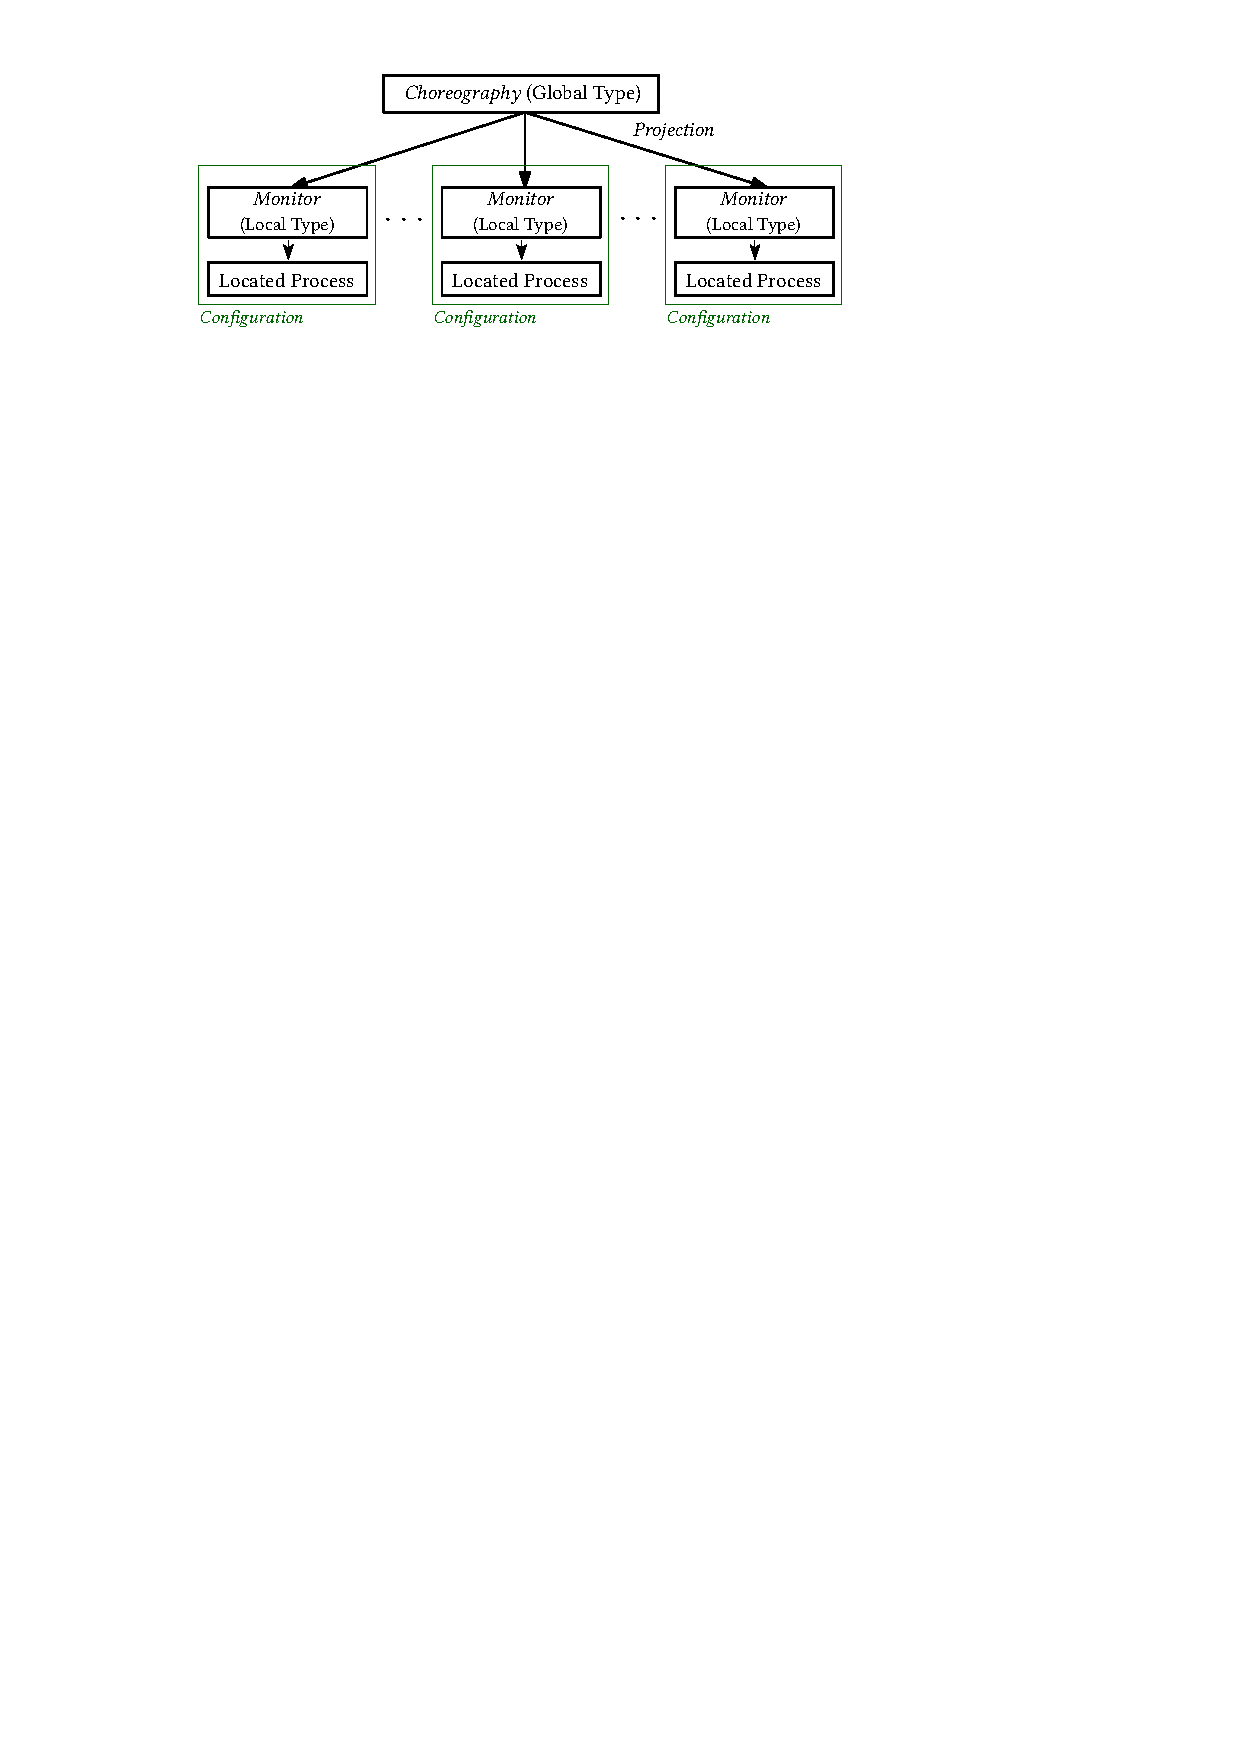
\includegraphics[width=8.7cm]{./img/figmodel.pdf}
\end{center}
\vspace{-4mm}
\caption{Our process model of multiparty communications.}\label{f:model}
\end{figure}
Fig.~\ref{f:model} depicts the ingredients of our
two-level model of \emph{choreographies} and \emph{configurations/processes}, given in~\cite{DBLP:conf/ppdp/MezzinaP17}.
Choreographies are defined in terms of \emph{global types}, which describe a protocol among two or more participants. 
A global type can be \emph{projected} onto each participant so as to obtain 
its corresponding  \emph{local type}, i.e., a session type that abstracts a participant's contribution to the global protocol. 
(We often use `choreographies' and `global types' as synonyms.)
The semantics of global types is given in terms of forward and backward  transition systems (Fig.~\ref{f:gts}). 
There is a \emph{configuration} for each protocol participant: it includes a \emph{located process}
that 
 specifies asynchronous communication behavior, subject to a \emph{monitor}
that enables forward/backward steps at run-time
based on the local type.
The semantics of configurations is given in terms of forward and backward reduction relations (Figs.~\ref{fig:fw} and~\ref{fig:bk}).
In the following, we  use colors to improve readability:
elements in \fwcolor{blue} belong to a forward semantics;
elements in \bkcolor{red} belong to a backward semantics.
%Given this two-level setting, our goal will be that of connecting (i)~forward and backward steps at the (high) level of choreographic specifications, and (ii) forward and backward steps at the (low) level of configurations/processes. This will be content of 
%Theorem~\ref{t:corrgc}.

\subsection{Global and Local Types}

\subsubsection{Syntax}
Let us write $\p, \q, \gpart{r}, \pA, \pB \ldots$ to denote (protocol) \emph{participants}.
The syntax of global types ($G, G', \ldots$) and local types  ($T, T', \ldots$) is standard~\cite{HYC08} and defined as follows:
\begin{align*}
			G, G'  \bnfis & \gtcom{p}{q}{U}{G} %\bnfbar 
			\sbnfbar
			\gtcho{p}{q}{\lbl_i}{G_i} %\\
			\sbnfbar %& 
			\mu X. G \sbnfbar X \sbnfbar \gend \\
			U, U'  \bnfis & \bool \sbnfbar \nat \sbnfbar \cdots %\bnfbar T 
			\sbnfbar \shot{T} \\
	    	T, T'  \bnfis & \ltout{p}{U}{T} \sbnfbar \ltinp{p}{U}{T} %\\
		  \sbnfbar %& 
		  \ltsel{p}{\lbl_i}{T_i}{i}{I} \sbnfbar \ltbra{p}{\lbl_i}{T_i}{i}{I}  
		 %\lsend{p}{\lbl_i}{U_i}{T_i} \bnfbar \lrecv{q}{\lbl_i}{U_i}{T_i} \bnfbar 
		\sbnfbar  \mu X. T \sbnfbar X \sbnfbar \lend 
\end{align*}
\noindent
Global type $\gtcom{p}{q}{U}{G}$ says that \p may send a value of type $U$ to \q, and then continue as $G$.
Given a finite index set $I$ and pairwise different \emph{labels} $\lbl_i$, global type $\gtcho{p}{q}{\lbl_i}{G_i}$ specifies that  \p may choose  label $\lbl_i$, communicate this selection to \q, and then continue as $G_i$.
In these two types %thus denote direct communications; 
we assume that $\p \neq \q$.
For the sake of presentation, here 
we do not consider labeled choices in global types; these can be easily accommodated---see \S\,\ref{s:ext} and~\cite{MezzinaP17arxiv}.
Global %types include also 
recursive and terminated protocols are denoted $\mu X. G$ and $\gend$, respectively.
We write $\parties{G}$ to denote the set of participants in $G$.
Value types $U$ include basic first-order values (constants),   but also \emph{higher-order} values: abstractions from names to processes. 
(We write $\Proc$ to denote the type of processes.)
Local types 
%abstract the behavior of individual participants. Types 
$\ltout{p}{U}{T}$ and $\ltinp{p}{U}{T}$ denote, respectively, an output and input of value of type $U$ by \p.
\added{We use  $\alpha$ to denote type prefixes  $\typeIn{\p}{U}$, $\typeOut{\p}{U}$.}
Type $\ltbra{p}{\lbl_i}{T_i}{i}{I}$ says that \p 
offers different behaviors, available as labeled alternatives;
conversely, type $\ltsel{\p}{\lbl_i}{T_i}{i}{I}$ 
says that \p may select one of such alternatives.
 Terminated and recursive local types are denoted $\lend$ and $\mu X. T$, respectively. 

As usual, we consider only recursive types $\mu X. G$ (and $\mu X. T$) in which $X$ occurs guarded in $G$ (and $T$).
 We shall take an equi-recursive view of (global and local) types, and so we consider two  types with the same regular tree as equal.
 
Global and local types are related by  \emph{projection}:
following~\cite{HYC08},
the projection of global type $G$ onto participant $\gpart{r}$, written $\tproj{G}{\gpart{r}}$, is defined in Fig.~\ref{f:proj}. 
\modif{Intuitively, $\tproj{G}{\gpart{r}}$ denotes the (local) contribution of   $\gpart{r}$ to the overall choreographic behavior that $G$ declaratively specifies.
As such, the projection of a directed communication $\gtcom{p}{q}{U}{G'}$ onto $\gpart{r}$ depends on
$\gpart{r}$'s involvement, which is reflected locally as an input or output local type (if $\gpart{r}$ is indeed involved) or 
as the terminated local protocol (otherwise). The projection of 
recursive choreographies follows a similar principle; recursive variables and the terminated choreography are projected as expected.}
%\modif{The projection  $\tproj{G}{\p}$ extrapolates the overall (local) behaviour of participant $\p$ from the global type G: if $p$ is involved into a communication from a global point of view then this is also reflected into its local type. Recursive type definitions, recursive variables and terminated  protocol are translated into the corresponding local ones.} 
\added{Projection for $\gtcho{p}{q}{l_i}{G_i}$ is noteworthy: 
the projections of the participants not involved in the choice (different from $\p, \q$) should correspond to the same identical local type.}
\begin{figure}[t!]
{%\small
\begin{align*}
\tproj{(\gtcom{p}{q}{U}{G})}{\gpart{r}} & = 
\begin{cases}
\ltout{\q}{U}{(\tproj{G}{\gpart{r}})} & \text{if $\gpart{r} = \gpart{p}$} \\
\ltinp{\p}{U}{(\tproj{G}{\gpart{r}})} & \text{if $\gpart{r} = \gpart{q}$} \\
(\tproj{G}{\gpart{r}}) &  \text{if $\gpart{r} \neq \gpart{q}, \gpart{r} \neq \gpart{p}$}
\end{cases}
\\
\tproj{(\gtcho{p}{q}{l_i}{G_i})}{\gpart{r}}  
& 
\erase{= 
\begin{cases}
\ltsel{\q}{\lbl_i}{(\tproj{G_i}{\gpart{r}})}{i}{I}  & \text{ if $\gpart{r} = \gpart{p}$} \\
\ltbra{\p}{\lbl_i}{\tproj{G_i}{\gpart{r}}}{i}{I}  & \text{ if $\gpart{r} = \gpart{q}$} \\
(\tproj{{G_1}}{\gpart{r}}) &  \text{ if $\gpart{r} \neq \gpart{q}, \gpart{r} \neq \gpart{p}$ and} \\ 
& \text{~~$\forall i, j \in I. \tproj{{G_i}}{\gpart{r}} = \tproj{{G_j}}{\gpart{r}}$}
\end{cases}
}
\\
\tproj{(\mu X. G)}{\gpart{r}} &= 
\begin{cases}
\mu X. \tproj{G}{\gpart{r}} & \text{if $\gpart{r}$ occurs in $G$}
\\
\lend & \text{otherwise}
\end{cases}
\\
\tproj{X}{\gpart{r}} & = X
\qquad
\tproj{\gend}{\gpart{r}} = \lend
\end{align*}
}
\vspace{-4mm}
\caption{Projection of a global type $G$ onto a participant $\gpart{r}$.\label{f:proj}}
\end{figure}

\subsubsection{Semantics of Choreographies}\label{ss:chore}
\begin{figure}[t!]
{%\small
\begin{mathpar}
\inferrule*[left=\fwcolor{(FVal1)}]{}
{\ctx{G}[ \past \gtcom{p}{q}{U}{G}] 
\fwg 
\ctx{G}[\gtcom{p}{\!\!\past q}{U}{G} ]}
\\
\inferrule*[left=\fwcolor{(FVal2)}]{}
{\ctx{G}[  \gtcom{p}{\!\!\past q}{U}{G}] 
\fwg 
\ctx{G}[\gtcom{p}{q}{U}{\past G} ]}
%\\
\\
\inferrule*[left=\fwcolor{(FCho1)}]{}
{
%\begin{array}{c}
\ctx{G}[\past \gtcho{p}{q}{l_i}{G_i}] 
\fwg  
\ctx{G}[\gpart{p}\to\!\!\past\gpart{q}:\{\lbl_i:G_i \,;\, \lbl_j:G_j\}_{i \in I\setminus j} ] 
%\end{array}
}
\\
%\\
\inferrule*[left=\fwcolor{(FCho2)}]{}
{
%\begin{array}{c}
\ctx{G}[\gpart{p}\to\!\!\past\gpart{q}:\{\lbl_i:G_i \,;\, \lbl_j:G_j\}_{i \in I\setminus j} ] 
\fwg
\ctx{G}[\gpart{p}\to\gpart{q}:\{\lbl_i:G_i \,;\, \lbl_j:\past G_j\}_{i \in I\setminus j} ] 
%\end{array}
}
%
\\
%%
\inferrule*[left=\bkcolor{(BVal1)}]{}
{\ctx{G}[\gtcom{p}{\!\!\past q}{U}{G} ]
\bkg
\ctx{G}[ \past \gtcom{p}{q}{U}{G}] 
}
\\
\inferrule*[left=\bkcolor{(BVal2)}]{}
{
\ctx{G}[\gtcom{p}{q}{U}{\past G} ]
\bkg
\ctx{G}[  \gtcom{p}{\!\!\past q}{U}{G}] 
}
\\
\inferrule*[left=\bkcolor{(BCho1)}]{}
{
%\begin{array}{c}
\ctx{G}[\gpart{p}\to\!\!\past\gpart{q}:\{\lbl_i:G_i \,;\, \lbl_j:G_j\}_{i \in I\setminus j} ] 
%\qquad \qquad
%\\
%\qquad \qquad
\bkg  
\ctx{G}[\past \gpart{p}\to\gpart{q}:\{\lbl_i:G_i \,;\, \lbl_j:G_j\}_{i \in I\setminus j} ]
%\end{array}
}
\\
\inferrule*[left=\bkcolor{(BCho2)}]{}
{
%\begin{array}{c}
\ctx{G}[\gpart{p}\to\gpart{q}:\{\lbl_i:G_i \,;\, \lbl_j:\past G_j\}_{i \in I\setminus j} ]
%\qquad \qquad
%\\
%\qquad \qquad
\bkg 
\ctx{G}[\gpart{p}\to\!\!\past\gpart{q}:\{\lbl_i:G_i \,;\, \lbl_j:G_j\}_{i \in I\setminus j} ] 
%\end{array}
}

\end{mathpar}
}
\vspace{-4mm}
\caption{Semantics of Global Types (Forward \& Backwards).\label{f:gts}}
\label{fig:prot_sem}
\end{figure}

The semantics of global types (Fig.~\ref{fig:prot_sem})
comprises forward and backward transition rules. 
%\jp{Indeed, our semantics seems more like an ``unlabeled LTS''. Could it be that labels will be useful later on?}
To express backward steps, we require some auxiliary notions.
We use \emph{global contexts}, ranged over by $\ctx{G}, \ctx{G}', \ldots$ with holes $\bullet$,  to record
previous actions, including the choices discarded and committed:
%\begin{center}
$$
\ctx{G}
\bnfis   
\bullet 
\sbnfbar  
\ctx{G}[\gtcom{p}{q}{U}{\ctx G}]
\sbnfbar
\ctx{G}[\gpart{p}\to\gpart{q}:\{\lbl_i:G_i \,;\, \lbl_j:\ctx{G}\}_{i \in I\setminus j} ]
$$
%\end{center}
We also use \emph{global types with history}, ranged over by $\mathsf{H}, \mathsf{H}', \ldots$, 
  to record the current protocol state. 
This state is denoted by the \emph{cursor}~$\past$, which we introduced in~\cite{DBLP:journals/corr/MezzinaP16}:
\begin{align*}
			\mathsf{H}, \mathsf{H}'  \bnfis & 			\past G \sbnfbar	G \past 
			\sbnfbar 
			\gtcom{p}{\!\!\past q}{U}{G} 
			\sbnfbar 
			\gtcom{p}{q}{U}{\past G} 
			\\\sbnfbar & 
			\gpart{p}\to\!\!\past\gpart{q}:\{\lbl_i:G_i \,;\, \lbl_j:G_j\}_{i \in I\setminus j} 
			\\ \sbnfbar & 
 			\gpart{p}\to\gpart{q}:\{\lbl_i:G_i \,;\, \lbl_j:\past G_j\}_{i \in I\setminus j}  
\end{align*}
%Projection and notation $\parties{\cdot}$ extend easily to global types $\gth{H}$ (cf. Fig.~\ref{f:projext}).
%Notation $\parties{\cdot}$ extends easily to global types $\gth{H}$.
Intuitively,  directed exchanges such as $\gtcom{p}{q}{U}{G}$ have three \emph{intermediate states},
characterized by the decoupled involvement of \p and \q in the intended asynchronous model.
The \emph{first state}, denoted $\past \gtcom{p}{q}{U}{G}$, describes the situation prior to the exchange.
The \emph{second state} represents the point in which \p has sent a value of type $U$ but this message has not yet
reached \q; this is denoted $\gtcom{p}{\!\!\past q}{U}{G}$.
The \emph{third state} represents the point in which \q has received the message from \p and
the continuation $G$ is ready to execute; this is denoted by $\gtcom{p}{q}{U}{\past G}$.
\modif{Using these intermediate states is central to precisely characterize the intended asynchronous semantics for processes.}
These intuitions extend to $\gtcho{p}{q}{l_i}{G_i}$, with the following caveat:
the second state should distinguish the choice made by $\p$ from the discarded alternatives; 
  we write $\gpart{p}\to\!\!\past\gpart{q}:\{\lbl_i:G_i \,;\, \lbl_j:G_j\}_{i \in I\setminus j}$ to describe that $\p$ has selected $\lbl_j$ and that this choice is still to be received by \q. Once this occurs, a state
  $\gpart{p}\to\gpart{q}:\{\lbl_i:G_i \,;\, \lbl_j:\past G_j\}_{i \in I\setminus j}$ is reached.

These  intuitions come in handy to describe the forward and backward transition rules
in Fig.~\ref{fig:prot_sem}. 
For a forward directed exchange of a value, 
Rule~\fwcolor{\textsc{(FVal1)}} formalizes the transition from the first   to the second state;
Rule~\fwcolor{\textsc{(FVal2)}} denotes the transition from the second to the third state.
Rules~\fwcolor{\textsc{(FCho1)}} and~\fwcolor{\textsc{(FCho2)}} are their analogues for the forward directed communication of a label.
Rules~\bkcolor{\textsc{(BVal1)}} and~\bkcolor{\textsc{(BVal2)}} undo the step performed by 
Rules~\fwcolor{\textsc{(FVal1)}} and~\fwcolor{\textsc{(FVal2)}}, respectively. 
\erase{Also, 
Rules~\bkcolor{\textsc{(BCho1)}} and~\bkcolor{\textsc{(BCho2)}} undo the step performed by 
Rules~\fwcolor{\textsc{(FCho1)}} and~\fwcolor{\textsc{(FCho2)}}, respectively.} 




\subsection{Processes and Configurations}
\label{subsec:syntax}

	\begin{figure}[t!]
	%{\small
		\begin{align*}
			u,w  \bnfis& n \sbnfbar x,y,z
			\qquad \quad
			n,n' \bnfis a,b \sbnfbar \ep{s}{\p}%, \dual{s} 
			\\
			 {v},  {v}'  \bnfis &  \true \sbnfbar \false \sbnfbar \cdots
			\\
			V,W \bnfis & {a,b} \sbnfbar  x,y,z \sbnfbar  v, v' \sbnfbar {\abs{x}{P}}
			\\%[1mm]
			P,Q
			 \bnfis &
			\bout{u}{V}{P}  \sbnfbar  \binp{u}{x}{P} 
			\erase{\sbnfbar \bsel{u}{\lbl_i. P_i}_{i\in I} \sbnfbar \bbra{u}{\lbl_i:P_i}_{i \in I}  }
			 %\\
			 %& 
			 \sbnfbar  P \Par Q \sbnfbar  {\rvar{X} \sbnfbar \recp{X}{P}} 
						\sbnfbar  
			 {\appl{V}{u}}  
			\sbnfbar \news{n} P \sbnfbar \inact
\\
M,N		 \bnfis &
\myloc{\loc}{\bout{a}{x}{P}}
\sbnfbar 
\myloc{\loc}{\binp{a}{x}{P}}
\sbnfbar 
M \Par N 
\sbnfbar 
\news{n} M
\sbnfbar 
\inact 
\\
& \sbnfbar 
\rtsyn{\np{\ep{\loc}{\p}}{\conf{\stack C}{P}}} %% running process
\sbnfbar 
\rtsyn{\monig{\ep{s}{\p}}{H}{\mytilde{x}}{\store}}  %% monitor
\\
& \sbnfbar 
\rtsyn{\codah{s}{h_i}{h_o}%{\restrict{\mytilde{\gpart{r}}}}
} % queue
\sbnfbar 
\rtsyn{\mem{k}{(\appl{V}{u})}{\loc}} % function
	\\
	\erase{\stack{C}, \stack{C}' \bnfis}  & \erase{\inact \sbnfbar \bsel{u}{\lbl_i. P_i}_{i\in I} \sbnfbar 
\bbra{u}{ \lbl_i:P_i}_{i \in I} \sbnfbar \stack{C}_1, \stack{C}_2}
\\
	\mytagg \bnfis & \rmark \sbnfbar \normark
\qquad
	 h \bnfis  \emp   \sbnfbar h \cons \valueq{\p}{\q}{m} \qquad m \bnfis V \erase{\sbnfbar \lbl}
\\[2mm]
%
    \alpha \bnfis &   \typeIn{\q}{U} \sbnfbar  \typeOut{\q}{U} 
    \\
	T,S		 \bnfis & \lend \sbnfbar	\alpha.S \erase{\sbnfbar \ltsel{\q}{\lbl_i}{S_i}{i}{I} \sbnfbar \ltbra{\q}{\lbl_i}{S_i}{i}{I}}
	\\
	H,K		 \bnfis & \past S \sbnfbar S\past \sbnfbar \alpha_1.\cdots .\alpha_n.\past S 
%	\\
%	& 
	\erase{\sbnfbar  
	\ltselp{\q}{\lbl_i:S_i \;;\; \lbl_j:H_j}{i}{I} \sbnfbar \ltbrap{\q}{\lbl_i:S_i \, , \, \lbl_j:H_j}{i}{I}}
		\end{align*}
		\vspace{-4mm}
	\caption{\newjb{Syntax of processes $P, Q$, configurations $M, N$, 
	  \erase{stacks $\stack{C}, \stack{C}'$, }
	local types $T, S$, local types with history $H, K$.
    Constructs given in \rtsyn{\text{boxes}} appear only at run-time.}}
	\label{fig:syntax}
%	\vspace{-1mm}
\end{figure}


\subsubsection{Syntax}
The syntax of processes and configurations is given in \figref{fig:syntax}.
For processes $P, Q, \ldots$ we
follow closely the syntax of \HOp, the core higher-order session $\pi$-calculus~\cite{KPY2016}.
%(In turn, \HOp is a subcalculus of the higher-order language studied  in~\cite{tlca07}.) 
The syntax of configurations builds upon that of processes.
%Next, we describe all these syntactic elements.

%\myparagraph{Values}
\emph{Names} $a,b,c$ (resp.~$s, s'$) 
range over shared (resp. session) names. 
We use session names indexed by  {participants}, denoted $\ep{s}{\p}, \ep{s}{\q}$. 
Names $n, m$ are session or shared names.
\added{First-order values  $v, v'$ include base values and constants.}
%Dual endpoints are $\dual{n}$ with $\dual{\dual{s}} = s$ and $\dual{a} = a$.
%We define the dual operation over names $n$ as $\dual{n}$ with
%$\dual{\dual{s}} = s$ and $\dual{a} = a$.
%Intuitively, names $s$ and $\dual{s}$ are dual (two) \emph{endpoints} while 
%shared names represent shared (non-deterministic) points. 
Variables are denoted by $x, y$, 
and recursive variables are denoted by $\varp{X}, \varp{Y}$.
The syntax of values $V$ includes shared names, first-order values, but also 
name abstractions (higher-order values)
$\abs{x}{P}$,   where $P$ is a process.
\added{As shown in~\cite{KPY2016}, abstraction passing suffices to express name passing (\emph{delegation}).}

Process terms include   prefixes for sending and receiving values $V$, written 
$\bout{u}{V} P$ and $\binp{u}{x} P$, respectively.
\erase{\added{Given a finite index set $I$,}
processes $\bsel{u}{\lbl_i. P_i}_{i\in I}$ and $\bbra{u}{l_i: P_i}_{i \in I}$ implement 
selection and branching (internal and external labeled choices, respectively). 
The selection  $\bsel{u}{\lbl_i. P_i}_{i\in I}$ is actually 
a non-deterministic choice over $I$.}
In an improvement with respect to~\cite{DBLP:journals/corr/MezzinaP16,MezzinaP17}, here we consider parallel composition of processes $P \Par Q$ 
and recursion $\recp{X}{P}$ (which binds the recursive variable $\varp{X}$ in process $P$).
%as we will discuss, adding these constructs entails challenges in the characterization of 
%causal consistent semantics (see next section).
Process 
$\appl{V}{u}$ 
is the application
which substitutes name $u$ on the abstraction~$V$. %; our semantics will ensure that $V$ is not a name.
Constructs for 
name restriction $\news{n} P$ and 
inaction $\inact$ are standard.
Session restriction $\news{s} P$ simultaneously binds all the participant endpoints in $P$.
We write $\fv{P}$ and $\fn{P}$ %, and $\sn{P}$ 
to denote the sets of free 
variables 
and names in $P$.
We assume $V$ in $\bout{u}{V}{P}$ does not include free recursive 
variables $\rvar{X}$.
If $\fv{P} = \emptyset$, we call $P$ {\em closed}.


%\\
Building upon processes, the syntax of configurations $M, N, \ldots$ includes constructs for \emph{session initiation}: 
\begin{enumerate}[$\bullet$]
\item configuration $\myloc{\loc}{\bout{a}{x}{P}}$ denotes the \emph{request} of a service identified with $a$ implemented in 
$P$ as $x$; 
\item conversely, configuration 
$\myloc{\loc}{\binp{a}{x}{P}}$
denotes service \emph{acceptance}. 
\end{enumerate}
In these constructs,  identifiers $\loc, \loc', \ldots$ denote    a  \emph{location} 
or  \emph{site} (as in, e.g., the distributed $\pi$-calculus~\cite{Hennessy07}).
Locations indexed by participants, useful in run-time expressions, are denoted $\ep{\loc}{\p}, \ep{\loc}{\q}$.
Configurations also include
inaction $\inact$, parallel composition  $M \Par N$,
name restriction $\news{n} M$, as well as
 the following \emph{run-time elements}: %, not part of ``source'' processes:
 
\begin{enumerate}[$\bullet$]
\item \emph{Running processes} are of the form $\np{\ep{\loc}{\p}}{\conf{\stack C}{P}}$, where $\loc$ is a location that 
hosts a process $P$ \erase{ and a \emph{(process) stack} $\stack{C}$} that implements participant $\p$.
\erase{A process stack is simply a list of processes, useful 
  to record/reinstate the discarded alternatives   in a labeled choice.}

\item \emph{Monitors} are of the form $\monig{\ep{s}{\p}}{H}{\mytilde{x}}{\store}$ 
where 
$s$ is the session being monitored, 
$\p$ is a participant,
$H$ is a history session type (i.e. a session type with ``memory''), 
$\mytilde{x}$ is a set of free variables, 
and the \emph{store} $\store$  records the value of such variables (see Def.~\ref{d:store}).
These four elements allow us to track the current protocol
and  state of the   monitored process.

Also, each monitor has a 
\emph{tag} $\mytagg$, which can be either \emph{empty} (denoted `$\normark$') or \emph{full} (denoted `$\rmark$'). 
When created all monitors have an empty tag; a full tag indicates that the running process associated to the monitor
is currently involved in a  decoupled reversible step.
\added{We often omit the empty tag 
(so we write 
$\moni{\ep{s}{\p}}{H}{\mytilde{x}}{\store}$ instead of 
$\hmoni{\ep{s}{\p}}{H}{\mytilde{x}}{\store}$)
and write $\monir{\ep{s}{\p}}{H}{\mytilde{x}}{\store}$ to emphasize the reversible (red) nature of a 
monitor with full tag.}


\item Following~\cite{DBLP:journals/mscs/KouzapasYHH16}, we have \emph{message queues}
of the form 
%$\codah{s}{h_i}{h_o}{\restrict{\mytilde{\p}}}$,
$\codah{s}{h_i}{h_o}$,
where $s$ is a session, $h_i$ is the input part of the queue, and $h_o$ is the output part of the queue.
Each queue contains messages of the form $\valueq{\p}{\q}{\anyv}$ (read: ``message $\anyv$ is sent from $\p$ to $\q$'').
As we will see, the effect of an output prefix in a process is to place the message in its corresponding output queue;
conversely, the effect of an input prefix is to obtain the first message from its input queue. 
\added{Messages in the queue are \textit{never consumed}: a process reads a message $\valueq{\p}{\q}{\anyv}$ by moving it from the (tail of) queue $h_o$ to the (top of) queue $h_i$. This way, the    delimiter `$\history$' distinguishes the \textit{past} of the queue from its \textit{future}.}

%Also, $\mytilde{\p}$ denotes a sequence of participant identities currently involved in a reversible step; when this sequence is empty, we  write  $\codah{s}{h_i}{h_o}{~}$ instead of $\codah{s}{h_i}{h_o}{\restrict{\epsilon}}$.

\item We use \emph{running functions} of the form $\mem{k}{(\appl{V}{u})}{\loc}$ to reverse
 applications $\appl{V}{u}$. While $k$ is a fresh identifier (key) for this term, $\loc$ is the location of 
the running process that contains the application.

\end{enumerate}

\noindent
We shall write $\procs$ and $\confs$ to indicate the set of processes and configurations, respectively. 
We call \emph{agent} an element of the set $\agents = \confs \cup \procs$. 
We let $P, Q$  to range over $\procs$; also, we use $L,M,N$ to range over $\confs$ and $A,B,C$ to range over $\agents$.
%; and closed $P$ without 
%free session names a {\em program}. 





\subsubsection{A Decoupled Semantics for Configurations}\label{ss:semconf}
We define a reduction relation on configurations, coupled with a structural congruence
 on processes and configurations.
Our reduction semantics defines a \emph{decoupled} treatment for reversing communication actions within a protocol.
Reduction is thus defined as $\red \subset \confs \times \confs$, whereas structural congruence is defined as $\scong\, \subset \procs^{2} \cup \confs^{2}$.  We require auxiliary definitions for \emph{contexts}, \emph{stores}, and \emph{type contexts}.

%\begin{definition}
\emph{Evaluation contexts} are configurations with one hole 
 `$\bullet$', as defined by the following grammar:
$$\ctx{E}\bnfis \bullet \sbnfbar M\Par \ctx{E} \sbnfbar \news{n}\, \ctx{E}$$
\emph{General contexts} $\ctx{C}$ are processes or configurations with one hole~$\bullet$: they are obtained  by replacing one occurrence of $\inact$ (either as a process or as a configuration) with $\bullet$.
%\end{definition}
%\noindent 
A congruence on processes and configurations is an equivalence  $\Re$ that is closed under general contexts: $P \,\Re\,  Q \Longrightarrow \myctx{C}{P}\,\Re\,  \myctx{C}{Q}$
and $M\Re N \Longrightarrow \myctx{C}{M}\,\Re\,  \myctx{C}{N}$.
We define $\equiv$  as the smallest congruence on processes and configurations
that satisfies the axioms in Fig.~\ref{fig:str}. \modif{Most axioms are standard and/or similar to those for the $\pi$-calculus~\cite{DBLP:conf/concur/SangiorgiW01}; the exception is $\np{\key{\loc}{\er}}{\conf{}{\news{a}P}} \scong \news{a}\np{\key{\loc}{\er}}{\conf{}{P}}$, which allows a bound name to cross the boundaries of a running process, 
thus relating processes and configurations.}
A relation $\Re$ on configurations is \emph{evaluation-closed} if it satisfies the   following rules:
\begin{mathpar}
 \inferrule*[left=(Ctx)]{M\,\Re\, N}{\myctx{E}{M}\,\Re\, \myctx{E}{N}} \and 
 \inferrule*[left=(Eqv)]{M \scong M' \and M' \,\Re\, N' \and N'\scong N}{M \,\Re\, N} \and 
\end{mathpar}

\begin{figure}[t!]
{%\small
\[
	\begin{array}{c}
		A \Par \inact \scong A
		\quad
		A \Par B \scong B \Par A
		\quad
		A \Par (B \Par C) \scong (A \Par B) \Par C
%		\\[1mm]
%		\quad 
		\\[1mm]
		A \Par \news{n} B \scong \news{n}(A \Par B)
		\ (n \notin \fn{P})
				\quad
		\news{n} \inact \scong \inact
		\\[1mm]
		\recp{X}{P} \scong P\subst{\recp{X}{P}}{\rvar{X}}
%		\\[1mm]
		\quad
		A \scong B \textrm{ if } A \scong_\alpha B\\
		\modif{\np{\key{\loc}{\er}}{\conf{\stack{C}}{\news{a}P}} \scong \news{a}\np{\key{\loc}{\er}}{\conf{\stack{C}}{P}} }\todo{check this}
%		\qquad
%		\dk{V \scong W \textrm{ if } V \scong_\alpha W
%\quad \abs{x}{P} \scong \abs{x}{Q} \textrm{ if } P \scong Q} 
%\quad
%	\np{\key{k}{i}}{(P \Par Q)} \scong \np{\key{k}{i}}{P} \Par \np{\key{k}{i}}{Q}
	\end{array}
\]
}
\vspace{-4mm}
\caption{Structural Congruence \todo{ADD SWAP ON QUEUES.}}
\label{fig:str}
\end{figure}
%To enable reversible labeled choices, we define the following class of \textit{choice contexts}:
%
%\begin{definition}[Choice context]
%\textit{Choice contexts} are processes with one hole, denoted ``$\bullet$'', and defined by the following grammar:
%%\begin{align*}
%%& \ctx{K},\ctx{H} \bnfis \quad \bullet \sbnfbar 
%%\bsel{u}{\lbl_w}\ctx{K} + \freeze{\sum_{i\in I\setminus w}\bsel{u}{\lbl_i} P_i} \sbnfbar 
%%\bbra{u}{\lbl_w:\ctx{K} \,,\, \freeze{\lbl_i:P_i}}_{i \in I\setminus w}
%%\end{align*}
%\begin{align*}
%& \ctx{K},\ctx{H} \bnfis \quad \bullet \sbnfbar 
%\ctx{K} + \freeze{\sum_{i\in I}\bsel{u}{\lbl_i} P_i} \sbnfbar 
%\bbra{u}{\ctx{K} \,,\, \freeze{\lbl_i:P_i}}_{i \in I}
%\end{align*}
%\end{definition}

%\noindent
The state of monitored processes is formalized as follows:

\begin{definition} \label{d:store}
A store $\store$ is a mapping from variables to values. Given a store $\store$, a variable $x$, and a value $V$, 
the \emph{update} $\store\upd{x}{V}$ and the 
 \emph{reverse update} $\rup{\store}{x}$ are defined as follows:
%\cm{we have to understand better this thing of all bound variables are different }
\begin{align*}
\store\upd{x}{V} & = \begin{cases}
\store\cup \{(x,V)\} &\text{ if } x\not\in \mathtt{dom}(\store) \\ 
\text{ undefined }  & \text{otherwise}
\end{cases} 
\\
\rup{\store}{x} & =  \begin{cases}
\store_1 &\text{ if } \store=\store_1\cup \{(x,V)\} \\ 
\store  & \text{otherwise}
\end{cases} 
\end{align*}
\end{definition}

\noindent Together with local types with history, the following notion of type context allows us to keep the current protocol state inside monitors: 
\begin{definition} 
\added{Let $k, k', \ldots$ denote fresh name identifiers.} We define 
\textit{type contexts} as (local) types with one hole, denoted ``$\bullet$'':
\begin{align*}
 \ctx{T},\ctx{S}   \bnfis  &  \bullet  \erase{\sbnfbar
 \q\btsel{\lbl_w:\ctx{T} \;;\; \lbl_i:S_i}_{i \in I\setminus w} \sbnfbar \q\btbra{\lbl_w:\ctx{T} \, , \, \lbl_i:S_i}_{i \in I\setminus w}}
 \\
  &\sbnfbar   \alpha.\ctx{T} \sbnfbar    k.\ctx{T} \sbnfbar (\loc,\loc_1,\loc_2).\ctx{T} 
\end{align*}
%\cm{They are no more types, because of $k$. Moreover we can compact $k$.T and $(k,k_1,k_2).T$ with $\tilde{k}$ but as to be an ordered list}
%\cm{Dire cosa sono $k$ and $\loc$}
\end{definition}
\added{\noindent Type contexts $k.\ctx{T}$ 
and $(\loc,\loc_1,\loc_2).\ctx{T}$ 
will be instrumental in formalizing reversibility of
name applications and thread spawning, respectively, which are not described by local types.}
This way, we will often have monitors of the form
$\monig{\ep{s}{\p}}{\myctxr{\ctx{T}}{\past S}}{\mytilde{x}}{\store}$, where  
$\ctx{T}$ and $S$ describe past and future protocol steps for $\p$, respectively.



%%% ==== START QUEUE EQUIVALENCE
%\begin{definition}[Equivalence on message queues]
%%\cm{Not sure we need this, otherwise we have that $a \rightarrow b; c \rightarrow d = c \rightarrow d; a \rightarrow b$}
%%\jp{I have modified this.}
%%Let $m$ stand for either $V$ or $\lbl$. 
%We define the structural equivalence on queues, denoted $\equivq$, as follows:
%\begin{align*}
%h\cons \valueq{\p_1}{\q_1}{\anyv_1} \cons \valueq{\p_2}{\q_2}{\anyv_2}  \cons h'
%\equivq 
%\qquad \qquad \qquad
%\\
%%\vspace{5mm}
%\qquad \qquad \qquad
%h\cons \valueq{\p_2}{\q_2}{\anyv_2} \cons \valueq{\p_1}{\q_1}{\anyv_1} \cons h'
%\end{align*}
%whenever $\p_1 \neq \p_2 \land \q_1 \neq \q_2$.
%Equivalence $\equivq$ extends  to configurations as expected.
%\end{definition}
%%% ==== END QUEUE EQUIVALENCE

\added{Abstraction passing can implement a form of \emph{session delegation}, for 
received abstractions $\abs{x}{P}$ can contain 
 free session names (indexed by participant identities). The following definition  identifies those names:}

\begin{definition}
Let 
$h$ and $\p$ be a queue 
and a participant, respectively. 
Also, let  
$\{\valueq{\q_1}{\p}{\abs{x_1}{P_1}}, \ldots, \valueq{\q_k}{\p}{\abs{x_k}{P_k}} \}$ 
 denote the (possibly empty) set of messages in $h$ containing abstractions sent to $\p$.
We write 
$\names{\p, h}$ to denote the set of participant identities occurring in 
$P_1, \ldots, P_k$.
%$\sn{P_1} \cup \cdots \cup \sn{P_k}$.}
\end{definition}




%%%%%%%%%%%%%%%%%%%%%%%%%%%%%%%%%%%%%%%%%%%%%%%%%%%%%%%%%%%%%%%%%%%%%%%
%%%%%%%%%%%%%%%%%%%%%%%%%%%%%%%%%%%%%%%%%%%%%%%%%%%%%%%%%%%%%%%%%%%%%%%
%%%%%%%%%%%%%%%%%%%%%%%%%%%%%%%%%%%%%%%%%%%%%%%%%%%%%%%%%%%%%%%%%%%%%%%


\begin{figure*}[t!]
{%\small
\begin{mathpar}
\inferrule*[left=\fwcolor{(Init)}]
{\parties{G}= \{\p_1,\cdots,\p_n\} \and 
\forall \gpart{p}_i\in \parties{G}. \, \tproj{G}{\gpart{p}_i} = T_{i}  } 
{ 
\!\!\!\!
\begin{array}{c}
\myloc{\loc_1}{\bout{a}{x_1:T_1}{P_{1}}} \Par 
\prod_{i \in \{2, \cdots, n\}}\myloc{\loc_i}{\binp{a}{x_i:T_i}{P_{i}}} 
\\
\fw
\\
\news{s} \left(\, 
\prod_{i \in\{1,\cdots,n\}} \np{\key{{\loc_{i}}}{\p_i}}{ \conf{\inact}{P_i\subst{\ep{s}{\p_i}}{x_i}}} \Par 
\moni{\ep{s}{\p_i}}{\past T_{i}}{x_i}{\upd{x_i}{a }}  \Par \codah{s}{\emp}{\emp}{}\right)\!\!\!\!
\end{array}
}
\and
%%%%%%%%%%%%%%%%%%%%%%%%%%%%%%%%%%%%%%%%%%%%%%%%%%%%%%%%%%%%%%%%%%%%%%%%%%%%%%%%%%%%
\inferrule*[left = \fwcolor{(Out)}]{ \p = \er \,\vee\, \p \in \names{\er, h_i} }{
\begin{array}{c}
\np{\key{\loc}{\er}}{ \conf{\stack{C}}{\bout{\ep{s}{\p}}{V}{P}}} \Par \moni{\ep{s}{\p}}{\myctxr{\ctx{T}}{\past  \ltout{\q}{U}{S}}}{\mytilde x}{\store} \Par \codah{s}{h_i}{h_o}{}  
\\
\fw 
\\
\np{\key{\loc}{\er}}{\conf{\stack{C}}{P}} \Par \moni{\ep{s}{\p}}{\myctxr{\ctx{T}}{ \ltoutp{\q}{U}{S}}}{\mytilde x}{\store} \Par 
\codah{s}{h_i}{h_o\cons \valueq{\p}{\q}{\myeval{V}{\sigma}}}{}
\end{array}
}
%%%%%%%%%%%%%%%%%%%%%%%%%%%%%%%%%%%%%%%%%%%%%%%%%%%%%%%%%%%%%%%%%%%%%%%%%%%%%%%%%%%%%
\and 
%
\inferrule*[left = \fwcolor{(In)}]{
\p = \er \,\vee\, \p \in \names{\er, h_i}
}
{\begin{array}{c}
\np{\key{\loc}{\er}}{\conf{\stack{C}}{\binp{\ep{s}{\p}}{y}{P}}} \Par \moni{\ep{s}{\p}}{\myctxr{\ctx{T}}{\past  \ltinp{\q}{U}{S}}}{\mytilde x}{\store} \Par \codah{s}{h_i}{\valueq{\q}{\p}{V}\cons h_o }{}
\\
\fw 
\\
\np{\key{\loc}{\er}}{\conf{\stack{C}}{P}} \Par \moni{\ep{s}{\p}}{ \myctxr{\ctx{T}}{\ltinpp{\q}{U}{S}}}{\mytilde x, y}{\store\upd{y}{V}} \Par 
\codah{s}{h_i\cons  \valueq{\q}{\p}{V}}{h_o }{} 
\end{array}
} 
%%%%%%%%%%%%%%%%%%%%%%%%%%%%%%%%%%%%%%%%%%%%%%%%%%%%%%%%%%%%%%%%%%%%%%%%%%%%%%%%%%%%%
\and
\erase{
\inferrule*[left=\fwcolor{(Sel)}]
{\p = \er \,\vee\, \p \in \names{\er, h_i}
\and
w\in J \and J\subseteq I }
{ 
\begin{array}{c}
\np{\key{\loc}{\er}}{ \conf{\stack C}{\bsel{\ep{s}{\p}}{\lbl_i. P_i}_{i\in I}}}  \Par 
\moni{\ep{s}{\p}}{\myctxr{\ctx{T}}{\past \ltsel{\q}{\lbl_j}{S_j}{j}{J}} }{\mytilde x}{\store} \Par \codah{s}{h_i}{h_o}{} \quad 
\\
\fw 
\\
\np{\key{\loc}{\er}}{ \conf{\stack C , \bsel{\ep{s}{\p}}{\lbl_i.P_i}_{i\in I\setminus w} }{P_w} }\Par 
\moni{\ep{s}{\p}}{ \myctxr{\ctx{T}}{ \ltselp{\q}{\lbl_j:S_j \, , \, \lbl_w:\past S_w}{j}{J\setminus w}} }{\mytilde x}{\store} 
%\\
%\quad \qquad
\Par 
\codah{s}{h_i}{h_o\cons  \valueq{\p}{\q}{\lbl_w} }{} 
\end{array} 
 }
 }
%%%%%%%%%%%%%%%%%%%%%%%%%%%%%%%%%%%%%%%%%%%%%%%%%%%%%%%%%%%%%%%%%%%%%%%%%%%%%%%%%%%%%
\and
\erase{
\inferrule*[left=\fwcolor{(Bra)}]{\p = \er \,\vee\, \p \in \names{\er, h_i} 
\and w\in I \and I\subseteq J }
{
\begin{array}{c}
\np{\key{\loc}{\er}}{ \conf { \stack C}{\bbra{\ep{s}{\p}}{\lbl_i:P_i}_{i \in I} } } \Par \moni{\ep{s}{\p}}{\myctxr{\ctx{T}}
{\past \ltbra{\q}{\lbl_j}{S_j}{j}{J}} }{\mytilde x}{\store} \Par \codah{s}{h_i}{\valueq{\q}{\p}{\lbl_w}\cons h_o}{} 
\\
\fw 
\\
\np{\key{\loc}{\er}}{ \conf { \stack C , \bbra{\ep{s}{\p}}{\lbl_i:P_i}_{i \in I\setminus w}}{ P_w} } \Par 
\moni{\ep{s}{\p}}{\myctxr{\ctx{T}}{\ltbrap{\q}{\lbl_j:S_j\,,\, \lbl_w:\past S_w}{j}{J\setminus w}} }{\mytilde x}{\store}
%\\
%\quad  \qquad 
\Par \codah{s}{h_i\cons  \valueq{\q}{\p}{\lbl_w}}{h_o}{}
\end{array}
 }
 }
%%%%%%%%%%%%%%%%%%%%%%%%%%%%%%%%%%%%%%%%%%%%%%%%%%%%%%%%%%%%%%%%%%%%%%%%%%%%%%%%%%%%%
\and
%
\inferrule*[left=\fwcolor{(Beta)}]{\myeval{V}{\sigma} =\abs{x}{P} }
{
\begin{array}{l}
\np{\key{\loc}{\p}}{\conf{\stack{C}}{(\appl{V}{w})}} \Par \moni{\ep{s}{\p}}{\myctxr{\ctx{T}}{\past S}}{\mytilde x}{\store} 
~\fw~ 
\news{k}\, \left( {\np{\key{\loc}{\p}}{\conf{\ctx{\stack {C}}}{P\subst{\myeval{w}{\sigma}}{x}}}}  \Par \mem{k}{(\appl{V}{w})}{\loc} \Par\moni{\ep{s}{\p}}{\myctxr{\ctx T}{ k. \past S}}{\mytilde x}{\store} \right)
\end{array}
}
%%%%%%%%%%%%%%%%%%%%%%%%%%%%%%%%%%%%%%%%%%%%%%%%%%%%%%%%%%%%%%%%%%%%%%%%%%%%%%%%%%%%%
\and
%
\inferrule[\fwcolor{(Spawn)}]{ }
{
\begin{array}{c}
\np{\key{\loc}{\p}}{\conf{\stack{C}}{P \Par Q}} \Par \moni{\ep{s}{\p}}{\myctxr{\ctx{T}}{\past S}}{\mytilde x}{\store} 
%\\
~\fw~ 
%\\
\news{\loc_1,\loc_2}\, \left( \np{\key{\loc}{\p}}{\conf{\stack{C}}{\inact}}  
\Par \np{\key{{\loc_1}}{\p}}{\conf{\inact}{P}}
\Par \np{\key{{\loc_2}}{\p}}{\conf{\inact}{Q}} 
\Par \moni{\ep{s}{\p}}{\myctxr{\ctx T}{ (\loc,\loc_1,\loc_2). \past S}}{\mytilde x}{\store} \right)
\end{array}
}

\end{mathpar}
}
%\vspace{-5mm}
\caption{Decoupled semantics for configurations: Forward reduction ($\fw$).}
\label{fig:fw}
\end{figure*}


%%%%%%%%%%%%%%%%%%%%%%%%%%%%%%%%%%%%%%%%%%%%%%%%%%%%%%%%%%%%%%%%%%%%%%%
%%%%%%%%%%%%%%%%%%%%%%%%%%%%%%%%%%%%%%%%%%%%%%%%%%%%%%%%%%%%%%%%%%%%%%%
%%%%%%%%%%%%%%%%%%%%%%%%%%%%%%%%%%%%%%%%%%%%%%%%%%%%%%%%%%%%%%%%%%%%%%%

\begin{figure*}[t!]
{%\small
\begin{mathpar}
\inferrule*[left=\bkcolor{(RInit)}]
{\parties{G}= \{\p_1,\cdots,\p_n\} \and 
\forall \gpart{p}_i\in \parties{G}. \, \tproj{G}{\gpart{p}_i} = T_{i} \and Q_i = P_{i}\subst{\ep{s}{\p_i}}{x_i} } 
{ 
\!\!\!\!
\begin{array}{c}
\news{s} \left(\, 
\prod_{i \in\{1,\cdots,n\}} \np{\key{{\loc_i}}{\p_i}}{ \conf{\inact}{Q_i}} \Par 
\hmoni{\ep{s}{\p_i}}{\past T_{i}}{x_i}{\upd{x_i}{a }}  \Par \codah{s}{\emp}{\emp}{}\right)
\\
~\bk~
\\
\myloc{\loc_1}{\bout{a}{x_1:T_1}{P_{1}}} \Par 
\prod_{i \in \{2, \cdots, n\}} \myloc{\loc_i}{\binp{a}{x_i:T_i}{P_i}}
\end{array}
\!\!\!\!
}
\and
%%%%%%%%%%%%%%%%%%%%%%%%%%%%%%%%%%%%%%%%%%%%%%%%%%%%%%%%%%%%%%%%%%%%%%%%%%%%%%%%%%%%%
\inferrule*[left=\bkcolor{(RollS)}]{ }{
\begin{array}{c}
\hmoni{\ep{s}{\p}}{ \myctxr{\ctx T}{\ltinpp{\q}{U}{T}}}{\mytilde x}{\store_1} \Par 
\hmoni{\ep{s}{\q}}{ \myctxr{\ctx S}{\ltoutp{\p}{U}{S}}}{\mytilde y}{\store_2} \Par 
%\codah{s}{h_i}{h_o}{\restrict{\mytilde{\gpart{r}}}}
\codah{s}{h_i}{h_o}
%\quad 
\\
\bk 
\\
\monir{\ep{s}{\p}}{ \myctxr{\ctx T}{\ltinpp{\q}{U}{T}}}{\mytilde x}{\store_1} \Par 
\monir{\ep{s}{\q}}{\myctxr{\ctx S}{\ltoutp{\p}{U}{S}}}{\mytilde y}{\store_2} \Par 
%\codah{s}{h_i}{h_o}{\restrict{\mytilde{\gpart{r}},\p,\q}}
\codah{s}{h_i}{h_o}
\end{array}
}
%%%%%%%%%%%%%%%%%%%%%%%%%%%%%%%%%%%%%%%%%%%%%%%%%%%%%%%%%%%%%%%%%%%%%%%%%%%%%%%%%%%%%%
\and 
%
\erase{
\inferrule*[left=\bkcolor{(RollC)}]{ }{
\begin{array}{c}
\hmoni{\ep{s}{\p}}{\myctxr{\ctx T}{\ltbrap{\q}{\lbl_z:\past S_z\,,\,\lbl_w:S_w}{z}{J\setminus w}}}{\mytilde x}{\store_1}  \Par 
\hmoni{\ep{s}{\q}}{\myctxr{\ctx S}{\ltselp{\p}{\lbl_z:\past S_z \, , \, \lbl_w: S_w}{z}{J\setminus w}}}{\mytilde y}{\store_2}  \Par 
%\codah{s}{h_i}{h_o}{\restrict{\mytilde{\gpart{r}}}}
\codah{s}{h_i}{h_o}
\\
\bk 
\\
\monir{\ep{s}{\p}}{ \myctxr{\ctx T}{\ltbrap{\q}{\lbl_z:\past S_z\,,\,\lbl_w:S_w}{z}{J\setminus w}}}{\mytilde x}{\store_1}  \Par 
\monir{\ep{s}{\q}}{\myctxr{\ctx S}{\ltselp{\p}{\lbl_z:\past S_z \, , \, \lbl_w: S_w}{z}{J\setminus w}}}{\mytilde y}{\store_2}  \Par 
%\codah{s}{h_1}{h_2}{\restrict{\mytilde{\gpart{r}},\p,\q}}
\codah{s}{h_i}{h_o}
\end{array}
}
}
%%%%%%%%%%%%%%%%%%%%%%%%%%%%%%%%%%%%%%%%%%%%%%%%%%%%%%%%%%%%%%%%%%%%%%%%%%%%%%%%%%%%%%
\and
%
\inferrule[\bkcolor{(ROut)}]{ \p = \er \,\vee\, \p \in \names{\er, h_i}}
{
\!\!\!\!
\begin{array}{l}
\np{\key{\loc}{\er}}{\conf{\stack C}{P}} \Par \monir{\ep{s}{\p}}{ \myctxr{\ctx T}{\ltoutp{\q}{U}{S}} }{\mytilde x}{\store}
\Par 
%\codah{s}{h_i}{(\p,\q,V)\cons h_o}{\restrict{\p,\mytilde{\gpart{r}}}}
\codah{s}{h_i}{(\p,\q,V)\cons h_o}
%\\
~\bk~
%\\
\np{\key{\loc}{\er}}{\conf{\stack C }{\bout{\ep{s}{\p}}{V}{P}}} \Par 
\hmoni{\ep{s}{\p}}{ \myctxr{\ctx T}{\past\ltout{\q}{U}{S}} }{\mytilde x}{\store}
 \Par %\codah{s}{h_i}{h_o}{\restrict{\mytilde{\gpart{r}}}}
 \codah{s}{h_i}{h_o}
\end{array}
\!\!\!\!
 }
%%%%%%%%%%%%%%%%%%%%%%%%%%%%%%%%%%%%%%%%%%%%%%%%%%%%%%%%%%%%%%%%%%%%%%%%%%%%%%%%%%%%%%
\and
%
\inferrule*[left=\bkcolor{(RIn)}]{ 
\p = \er \,\vee\, \p \in \names{\er, h_i}
}
{
\begin{array}{c}
\np{\key{\loc}{\er}}{\conf{\stack C}{P}} \Par 
\monir{\ep{s}{\p}}{ \myctxr{\ctx T} {\ltinpp{\q}{U}{S}} }{\mytilde x,y}{\store} \Par 
%\codah{s}{h_i\cons(\q,\p,V)}{h_o}{\restrict{\p,\mytilde{\gpart{r}}}}
\codah{s}{h_i\cons(\q,\p,V)}{h_o}
\\
\quad \bk
\\
\np{\key{\loc}{\er}}{\conf{\stack C} { \binp{\ep{s}{\p}}{y}{P}} } \Par 
\hmoni{\ep{s}{\p}}{ \myctxr{\ctx T}{\past\ltinp{\q}{U}{S}}}{\mytilde x}{\rup{\store}{y}}\Par %\codah{s}{h_i}{(\q,\p,V)\cons h_o}{\restrict{\mytilde{\gpart{r}}}}
\codah{s}{h_i}{(\q,\p,V)\cons h_o}
\end{array}
 }
%%%%%%%%%%%%%%%%%%%%%%%%%%%%%%%%%%%%%%%%%%%%%%%%%%%%%%%%%%%%%%%%%%%%%%%%%%%%%%%%%%%%%%
\and
\erase{
\inferrule*[left=\bkcolor{(RBra)}]
{ \p = \er \,\vee\, \p \in \names{\er, h_i} \and w \in I \and I\subseteq J} 
{
\begin{array}{c}
\np{\key{\loc}{\er}}{\conf{\stack C,\bbra{\ep{s}{\p}}{\lbl_i:P_i }_{i \in I\setminus\set{w}}}{P}
} \Par 
\monir{\ep{s}{\p}}{\myctxr{\ctx T}{\ltbrap{\q}{\lbl_j:S_j\,,\, \lbl_w:\past S_w}{j}{J\setminus w}} }{\mytilde x}{\store}
\Par 
%\codah{s}{h_i\cons  \valueq{\q}{\p}{\lbl_w}}{h_o}{\restrict{\p, \mytilde{\gpart{r}}}}
\codah{s}{h_i\cons  \valueq{\q}{\p}{\lbl_w}}{h_o}
\\
\quad \bk 
\\%[1mm]
\np{\key{\loc}{\er}}{ \conf{\stack C}{\bbra{\ep{s}{\p}}{\lbl_i:P_i, \lbl_w : P }_{i \in I\setminus\set{w}}}} \Par 
\hmoni{\ep{s}{\p}}{\myctxr{\ctx T}{\past\ltbra{\q}{\lbl_j}{S_j}{j}{J}} }{\mytilde x}{\store} 
\Par 
%\codah{s}{h_i}{\valueq{\q}{\p}{\lbl_w}\cons h_o}{\restrict{\mytilde{\gpart{r}}}}
\codah{s}{h_i}{\valueq{\q}{\p}{\lbl_w}\cons h_o}
\end{array}
 }}
\and 
%%%%%%%%%%%%%%%%%%%%%%%%%%%%%%%%%%%%%%%%%%%%%%%%%%%%%%%%%%%%%%%%%%%%%%%%%%%%%%%%%%%%%%
\erase{
\inferrule*[left=\bkcolor{(RSel)}]
{ \p = \er \,\vee\, \p \in \names{\er, h_i} \and w \in I \and I\subseteq J} 
{
\begin{array}{c}
\np{{\key{\loc}{\er}}}{ \conf{\stack C,\bsel{\ep{s}{\p}}{\lbl_i. P_i}_{i\in I} }{P}} \Par 
\monir{\ep{s}{\p}}{ \myctxr{\ctx T}{ \ltselp{\q}{\lbl_j:S_j \, , \, \lbl_w:\past S_w}{j}{J\setminus w} } }{\mytilde x}{\store}
\Par 
%\codah{s}{h_i}{\valueq{\p}{\q}{\lbl_w}\cons h_o}{\restrict{\p,\mytilde{\gpart{r}}}}
\codah{s}{h_i}{\valueq{\p}{\q}{\lbl_w}\cons h_o}
\\
\quad \bk 
\\
\np{{\key{\loc}{\er}}}{ \conf{\stack C}{ \bsel{\ep{s}{\p}}{\lbl_w. P} + \bsel{\ep{s}{\p}}{\lbl_i. P_i}_{i\in I} } } \Par 
\hmoni{\ep{s}{\p}}{ \myctxr{\ctx T}{ \past \ltsel{\q}{\lbl_j}{S_j}{j}{J} } }{\mytilde x}{\store} \Par 
%\codah{s}{h_i}{h_o}{\restrict{\mytilde{\gpart{r}}}}
\codah{s}{h_i}{h_o}
\end{array}
}
}
%%%%%%%%%%%%%%%%%%%%%%%%%%%%%%%%%%%%%%%%%%%%%%%%%%%%%%%%%%%%%%%%%%%%%%%%%%%%%%%%%%%%%%
\and
%
\inferrule*[left=\bkcolor{(RBeta)}]{ }
{
\begin{array}{l}
\news{k}\,\left( {\np{\key{\loc}{\p}}{\conf{\stack{C}}{Q} }}  \Par \mem{k}{(\appl{V}{w})}{\loc} 
\Par\moni{\ep{s}{\p}}{\myctxr{\ctx T}{ k. \past S}}{\mytilde x}{\store}
\right)
%\\
~\bk~ 
%\\
\np{\key{\loc}{\p}}{\conf{\stack{C}}{(\appl{V}{w})}} \Par 
\moni{\ep{s}{\p}}{\myctxr{\ctx{T}}{\past S}}{\mytilde x}{\store} 
\end{array} 
}
%%%%%%%%%%%%%%%%%%%%%%%%%%%%%%%%%%%%%%%%%%%%%%%%%%%%%%%%%%%%%%%%%%%%%%%%%%%%%%%%%%%%%%
 \and
\inferrule[\bkcolor{(RSpawn)}]{ }
{
\begin{array}{c}
\news{\loc_1,\loc_2}\, \left( {\np{\key{\loc}{\p}}{\conf{\stack{C}}{\inact}}}  
\Par \np{\key{{\loc_1}}{\p}}{\conf{\inact}{P}}
\Par \np{\key{{\loc_2}}{\p}}{\conf{\inact}{Q}} 
\Par \moni{\ep{s}{\p}}{\myctxr{\ctx T}{ (\loc,\loc_1,\loc_2). \past S}}{\mytilde x}{\store} \right)
%\\
~\bk~
%\\
\np{\key{\loc}{\p}}{\conf{\stack{C}}{P \Par Q}} \Par 
\moni{\ep{s}{\p}}{\myctxr{\ctx{T}}{\past S}}{\mytilde x}{\store}  
\end{array}
}

\end{mathpar}
}
%\vspace{-4mm}
\caption{Decoupled semantics for configurations: Backwards reduction ($\bk$).}
\label{fig:bk}
%\vspace{-3mm}
\end{figure*}

%\noindent 
The reduction relation $\red$ is defined as the union of %two relations: 
the forward and backward
reduction relations, denoted $\fw$  and $\bk$, respectively. That is, $\red\, = \fw \cup \bk$. Relations $\fw$ and 
$\bk$ are the smallest evaluation-closed relations satisfying the rules in Figs.~\ref{fig:fw} and~\ref{fig:bk}. We indicate with $ \trans{\red} $, $ \fws $, and $ \bks $  the reflexive and transitive closure of $\red$, $\fw$ and $\bk$, respectively.
%We write $M \red^k M'$ to denote a sequence of $k \geq 0$ reduction steps (if $k=0$ then $M = M'$)
We first discuss the forward reduction rules (Fig.~\ref{fig:fw}), omitting empty tags $\normark$:
% given in \ref{fig:fw} and \ref{fig:bk}.

\begin{enumerate}[$\fwcolor{\blacktriangleright}$]
\item Rule \fwcolor{\textsc{(Init)}} initiates a choreography  $G$ with $n$ participants.
Given the composition of one service request and $n-1$ service accepts (all along $a$, available in different locations~$\loc_i$),
this rule sets up the run-time elements:
running processes and  monitors---one for each participant, with empty tag (omitted)---and the empty session queue. 
A unique session identifier  ($s$ in the rule) is also created.
The processes are inserted in 
their respective running structures, and instantiated with an appropriate session name.
Similarly, the local types for each participant are inserted in their respective monitor, with the cursor $\past$ at the beginning.

\item Rule \fwcolor{\textsc{(Out)}} starts the output of value $V$ from $\p$ to $\q$. Given an output-prefixed process as running process,
and a monitor with a local type supporting an output action, reduction adds the message $\valueq{\p}{\q}{\myeval{V}{\sigma}}$ to the output part of the session queue (where $\sigma$ is the current store). Also, the cursor within the local type is moved accordingly.
In this rule (but also in several other rules), premise $\p = \er \,\vee\, \p \in \names{\er, h_i}$ allows performing actions on names previously received via abstraction passing.

\item Rule \fwcolor{\textsc{(In)}} allows a participant $\p$ to receive a value $V$ from $\q$: it 
simply takes the first element of the output part of the queue and places it in the input part.
The cursor of the local type and state in the  monitor for $\p$ are updated accordingly.

 
%\item 
\erase{Rule \fwcolor{\textsc{(Sel)}} is the forward rule for labeled selection, which in our case entails a non-deterministic choice between 
pairwise different labels indexed by $I$. %This is how our construct is more general than usual selection constructs.
We require that $I$ is contained in $J$, i.e., the set that indexes the choice according to the choreography. 
After reduction, the selected label ($\lbl_w$ in the rule) is added to the output part of the queue, and the continuation $P_w$ is kept in the running process;
to support reversibility,
alternatives different from $\lbl_w$ are stored in the stack $\stack{C}$ with their continuations.
The cursor is also appropriately updated in the  monitor.}

%\item 
\erase{Rule~\fwcolor{\textsc{(Bra)}} is similar to Rule \fwcolor{\textsc{(Sel)}}: it takes a message containing a label $\lbl_w$ as the first element in the output part of the queue, and places it into the input part. This entails a selection between the options indexed by $I$; the continuation $P_w$ is kept in the running process, and all those options different from $\lbl_w$ are kept in the stack. Also, the local type in the monitor is updated accordingly.
}
\item Rule~\fwcolor{\textsc{(Beta)}} handles name applications. Reduction  creates a fresh identifier ($k$ in the rule) for the running function, which keeps (i) the structure of the process prior to application, and (ii) the identifier of the running process that ``invokes'' the application. Notice that $k$ is recorded also in the monitor: this is necessary to undo applications in the proper order. To determine the actual abstraction and the name applied, we use   $\store$.

\item Rule~\fwcolor{\textsc{(Spawn)}} handles parallel composition. Location $\loc$ is ``split'' into running processes with fresh identifiers ($\loc_1, \loc_2$ in the rule). This split is recorded in the   monitor.
\end{enumerate}


\todo{ADD SIMPLE EXAMPLE (NOW IN APPENDIX) OF CHOICE CONTEXTS (FWD ONLY).}

\noindent
Now we comment on the backward rules (Fig.~\ref{fig:bk}) which, in most cases, change the monitor tags from $\normark$ into $\bkcolor{\rmark}$:

\begin{enumerate}[$\bkcolor{\blacktriangleleft}$]
\item Rule \bkcolor{\textsc{(RInit)}} undoes session establishment. It requires that local types for every participant are at the beginning of the protocol, and empty session queue and process stacks. Run-time elements are discarded; located service accept/requests are reinstated.

\item Rule~\bkcolor{\textsc{(RollS)}} starts to undo an input-output synchronization between $\p$ and $\q$. 
Enabled when there are complementary session types in the two monitors, this rule changes the monitor tags  from $\normark$ to $\bkcolor{\rmark}$. %, and marks  the queue with $\p$ and $\q$, to indicate that messages in the queue could now be moved between its input and output parts. 
This way, the undoing of input and output actions occurs in a decoupled way. 
%\item 
Rule \bkcolor{\textsc{(RollC)}} is the analog of~\bkcolor{\textsc{(RollS)}} but for synchronizations originated in labeled choices.

\item Rule \bkcolor{\textsc{(ROut)}} undoes an output. This is only possible for a  monitor tagged with $\bkcolor{\rmark}$, exploiting the first message in the input queue. After reduction, the process prefix is reinstated, the cursor is adjusted, the message is removed from the queue, 
the   monitor is tagged again with $\normark$.
%, and the identity of the involved participant ($\p$ in the rule) is removed from the  queue
%\item 
Rule \bkcolor{\textsc{(RIn)}} is the analog of Rule \bkcolor{\textsc{(ROut)}}. In this case, we also need to update the state of store $\store$. 
%\jp{Actually, it seems better to explain \textsc{(RollIn)} first and then \textsc{(RollOut)}.}

%\item 
\erase{Rule \bkcolor{\textsc{(RBra)}} undoes the input part of a labeled choice: the choice context is reinstated; the cursor is moved; the last message in the input part of the queue is moved to the output part. 
%; the identity of the participant ($\p$ in the rule) is removed from the queue; and the monitor is tagged again with $\normark$.
%\item 
Rule \bkcolor{\textsc{(RSel)}} is the analog of~\bkcolor{\textsc{(RBra)}}, but for the output part of the labeled choice. The non-deterministic   selection is reinstated.}

\item Rule \bkcolor{\textsc{(RBeta)}} undoes $\beta$-reduction, reinstating the application. The running function disappears, using the information in the 
  monitor ($k$ in the rule).
Rule~\bkcolor{\textsc{(RSpawn)}} undoes the spawn of a parallel thread, using the identifiers in the  monitor. 
%\jp{This rule will depend on what we decide for parallel inside processes, and session initiation.}
\end{enumerate}

\noindent
We now illustrate our reversible process model with an example.


\section{Our Haskell Implementation}

\section{Concluding Remarks and Future Work}
%
% ---- Bibliography ----
%
% BibTeX users should specify bibliography style 'splncs04'.
% References will then be sorted and formatted in the correct style.
%
 \bibliographystyle{splncs04}
 \bibliography{session,biblio}
%
\end{document}
